\chapter{Utilizzo}
\label{Utilizzo}
\section{Utilizzo dell'applicazione MegAlexa}
\label{UtilizzoApp}
\subsection{Creazione Workflow}
Per la creazione di un workflow seguire le seguenti istruzioni.\\
Al primo avvio dell'applicazione apparirà una schermata vuota, priva di \textit{workflow$_{G}$} come nella seguente immagine.
\begin{enumerate}
\item Cliccare sul tasto "+" per aggiungere un nuovo workflow;


	\begin{figure}[H]
		\centering
			\fbox{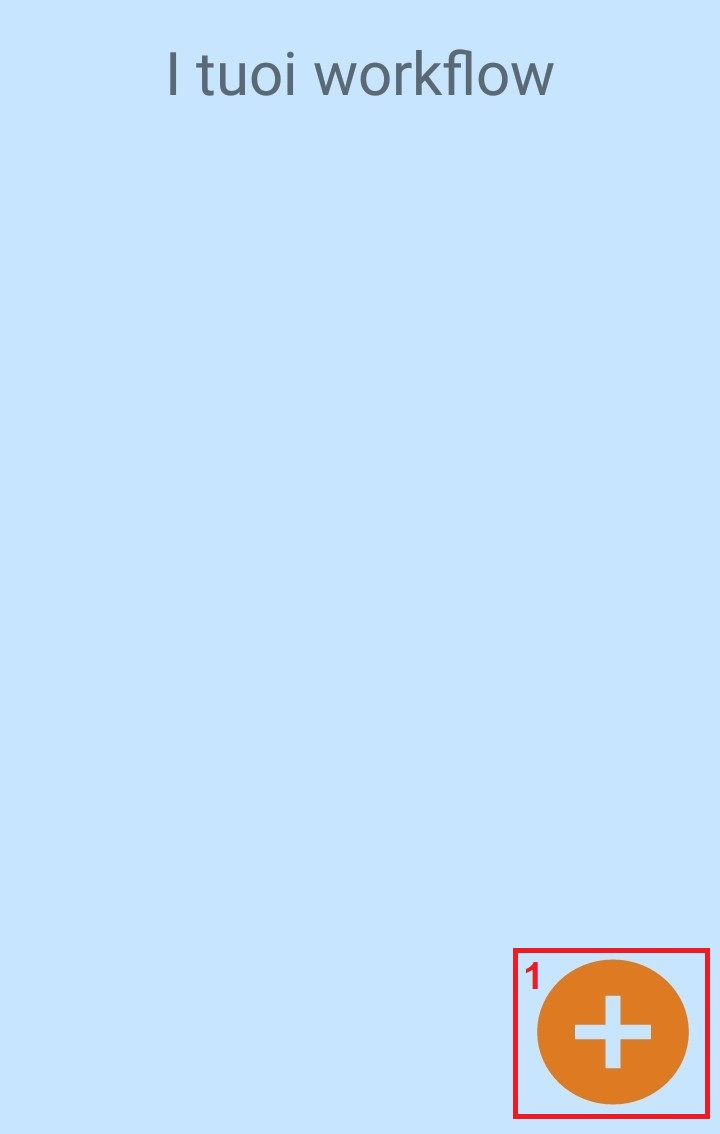
\includegraphics[width=0.35\textwidth]{images/HomeWorkflowEmpty.jpg}}
		\caption{Elenco workflow vuoto}
	\end{figure}


\item Inserire il nome del nuovo workflow nell'apposito campo di testo;\\
\textbf{NOTA BENE:} all'utente non è permesso creare due o più workflow con lo stesso nome;

	\begin{figure}[H]
		\centering
			\fbox{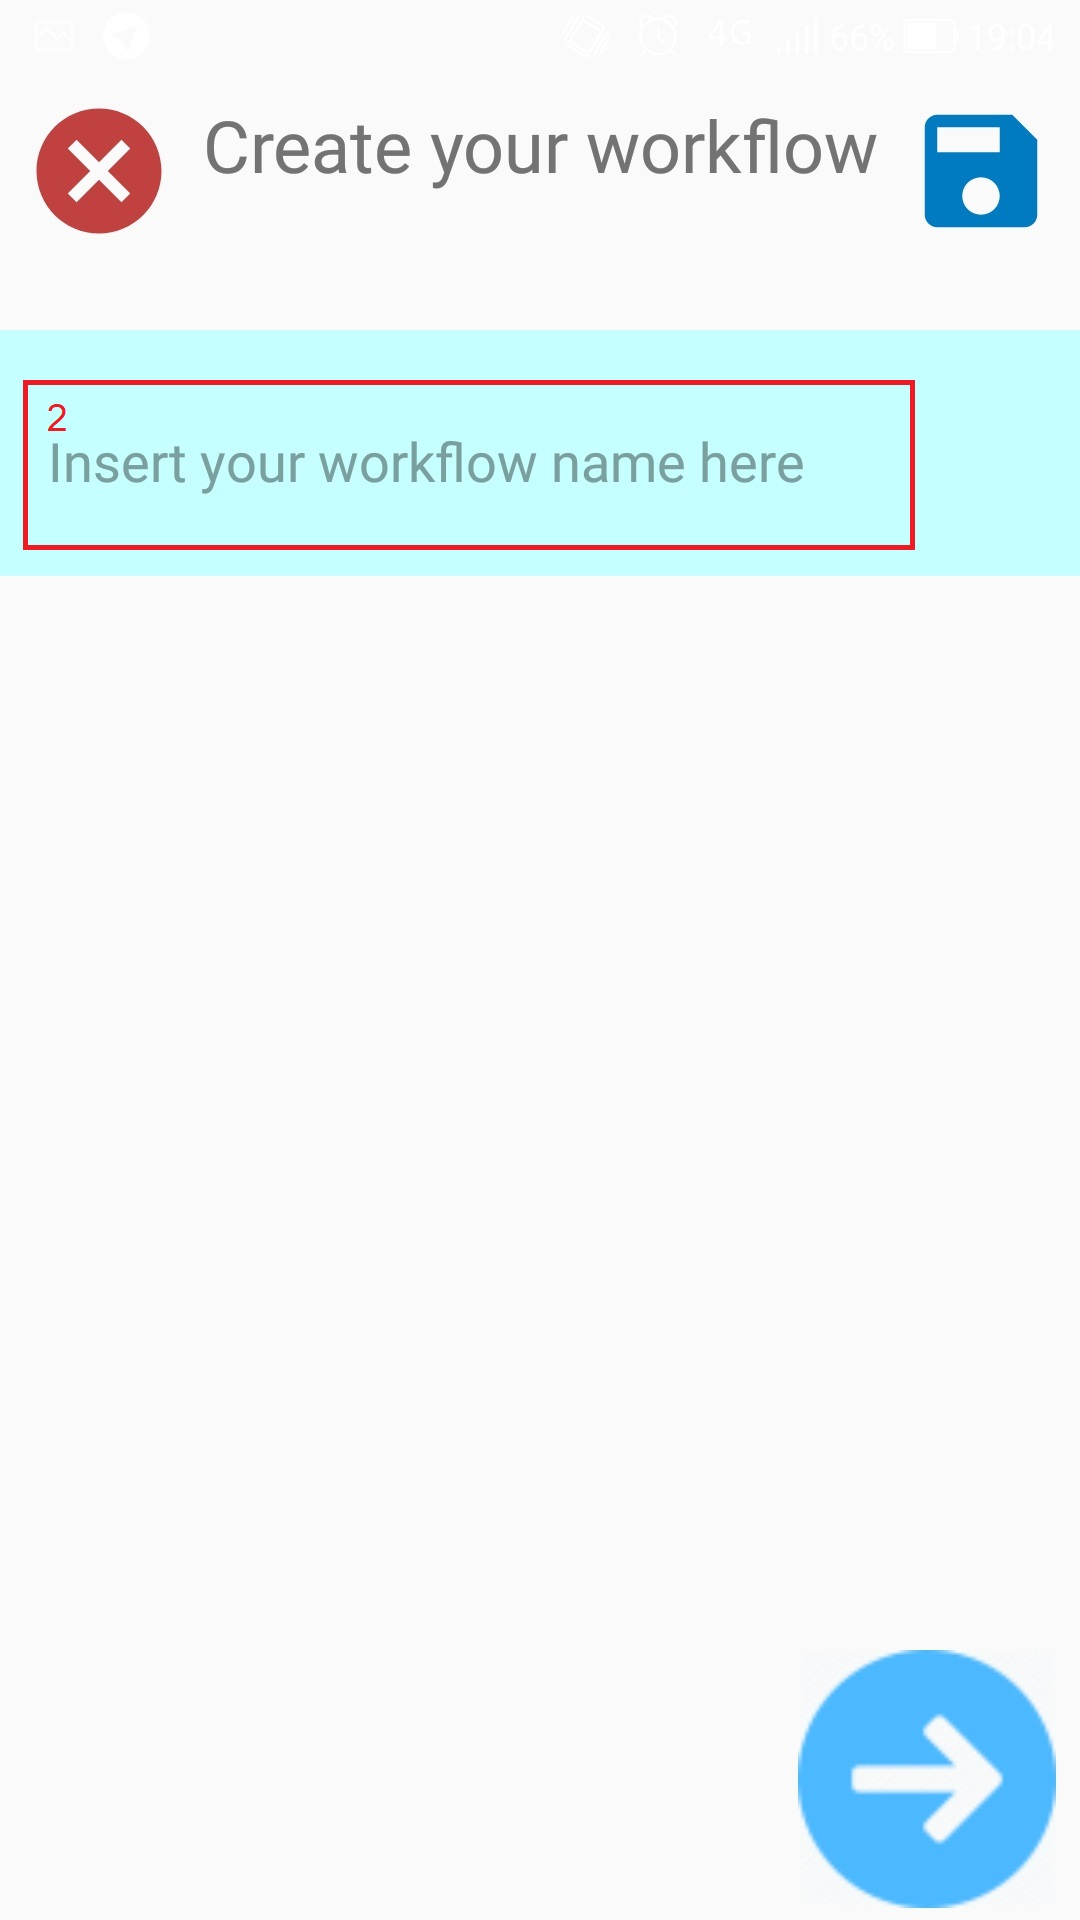
\includegraphics[width=0.5\textwidth]{images/AddWorkflow.jpg}}
		\caption{Schermata aggiunta workflow}
	\end{figure}

\newpage
\item Per aggiungere blocchi al workflow cliccare sulla freccia in basso a destra;

\begin{figure}[H]
	\centering
	\fbox{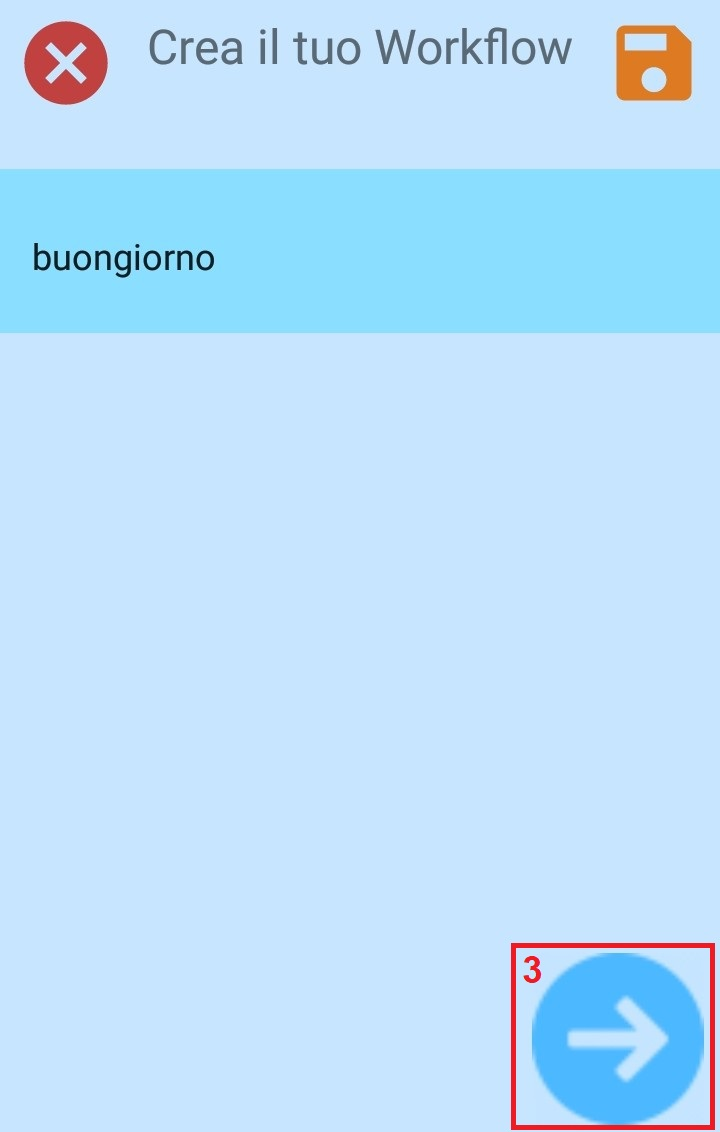
\includegraphics[width=0.5\textwidth]{images/Freccia.jpg}}
	\caption{Schermata aggiunta workflow}
\end{figure}

\newpage
\item Apparirà sulla schermata l'elenco dei blocchi che possono essere aggiunti.
Per aggiungere i blocchi che si desiderano seguire le istruzioni nel paragrafo successivo.
\begin{figure}[!ht]
	\centering
	\fbox{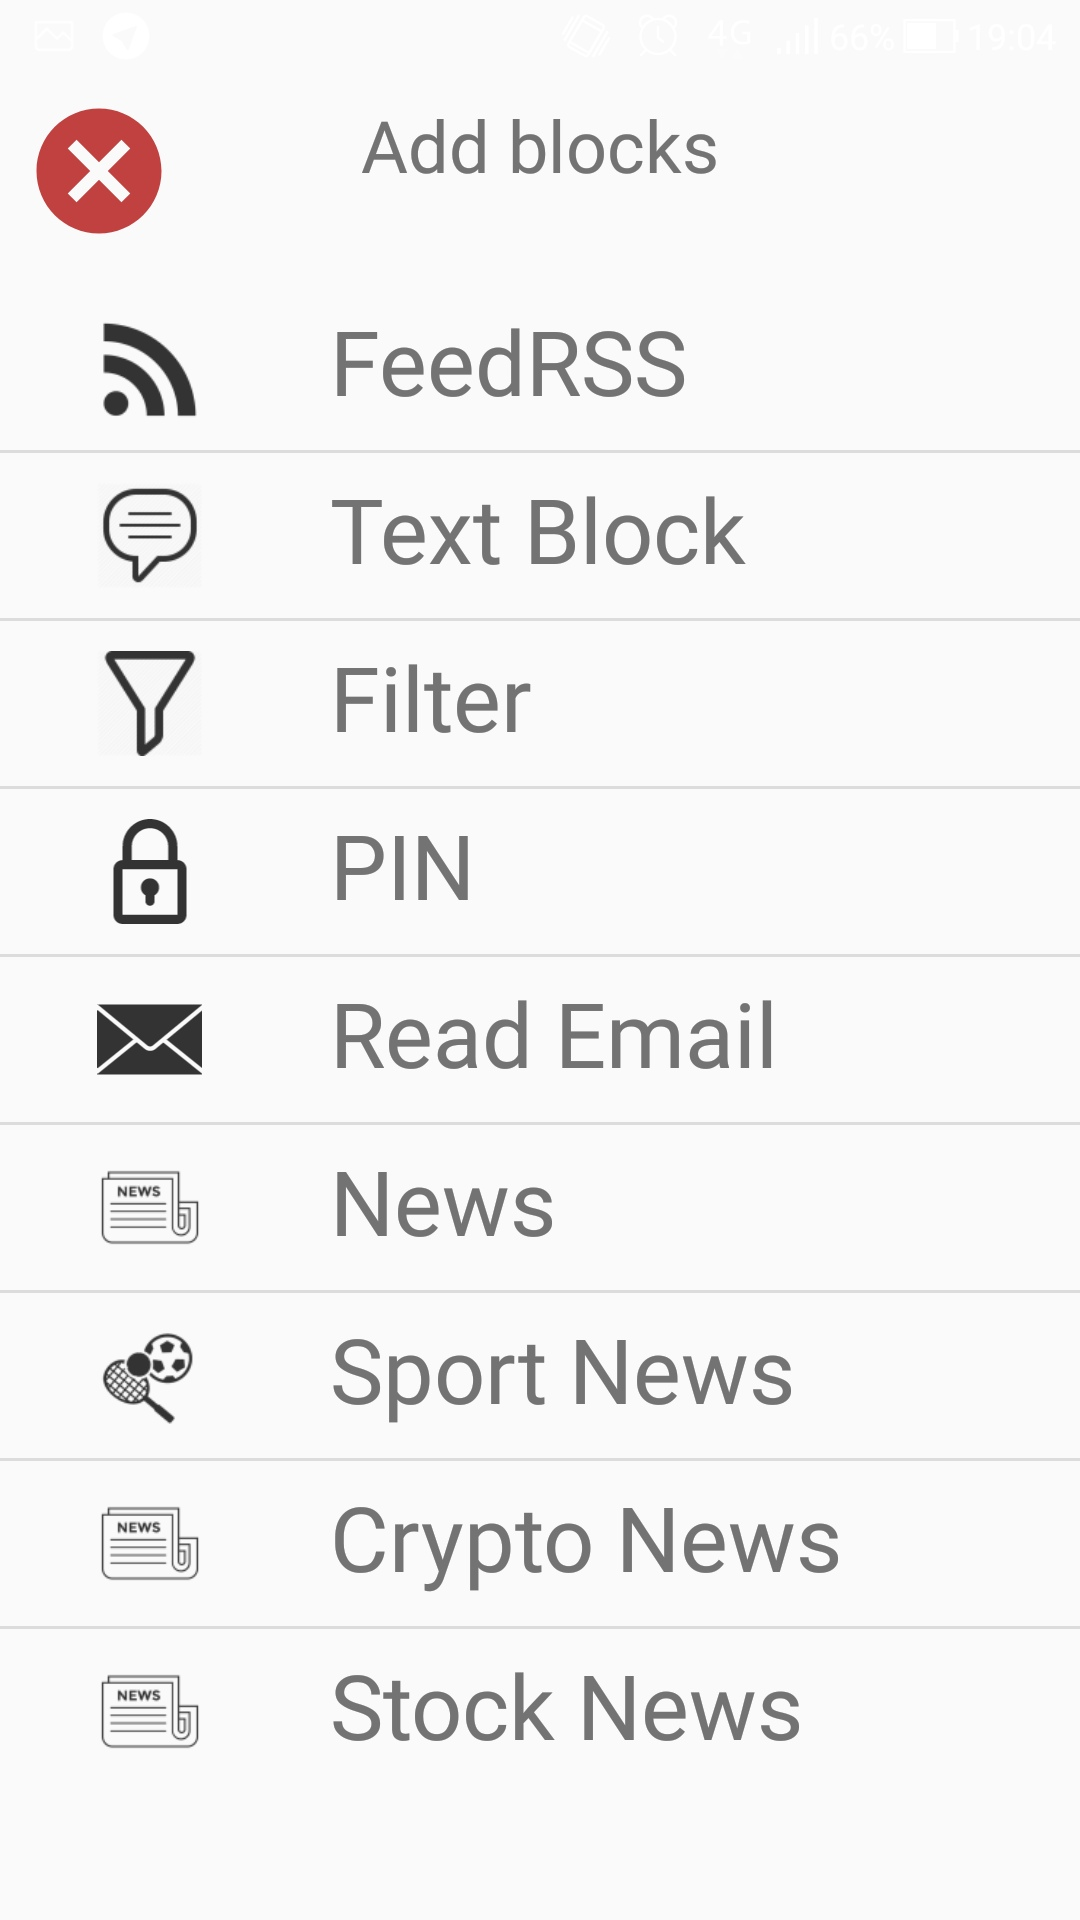
\includegraphics[width=0.35\textwidth]{images/ListBlocks.jpg}}
	\caption{Lista dei blocchi}
\end{figure}

\end{enumerate}

\newpage
\subsection{Aggiunta blocchi}
Segue una spiegazione dettagliata sulla configurazione e aggiunta di ogni blocco al \textit{workflow$_{G}$}.\\

\subsubsection{Blocco FeedRSS}
Questo blocco permette all'utente di inserire un qualsiasi feedRSS e successivamente far riprodurre al dispositivo Alexa il suo contenuto.
\begin{enumerate}
	\item Inserire nell'apposito campo di testo l'URL del feedRSS;
	\item Confermare e salvare cliccando sul pulsante "ADD" per aggiungere il blocco al workflow.
\begin{figure}[!ht]
	\centering
	\fbox{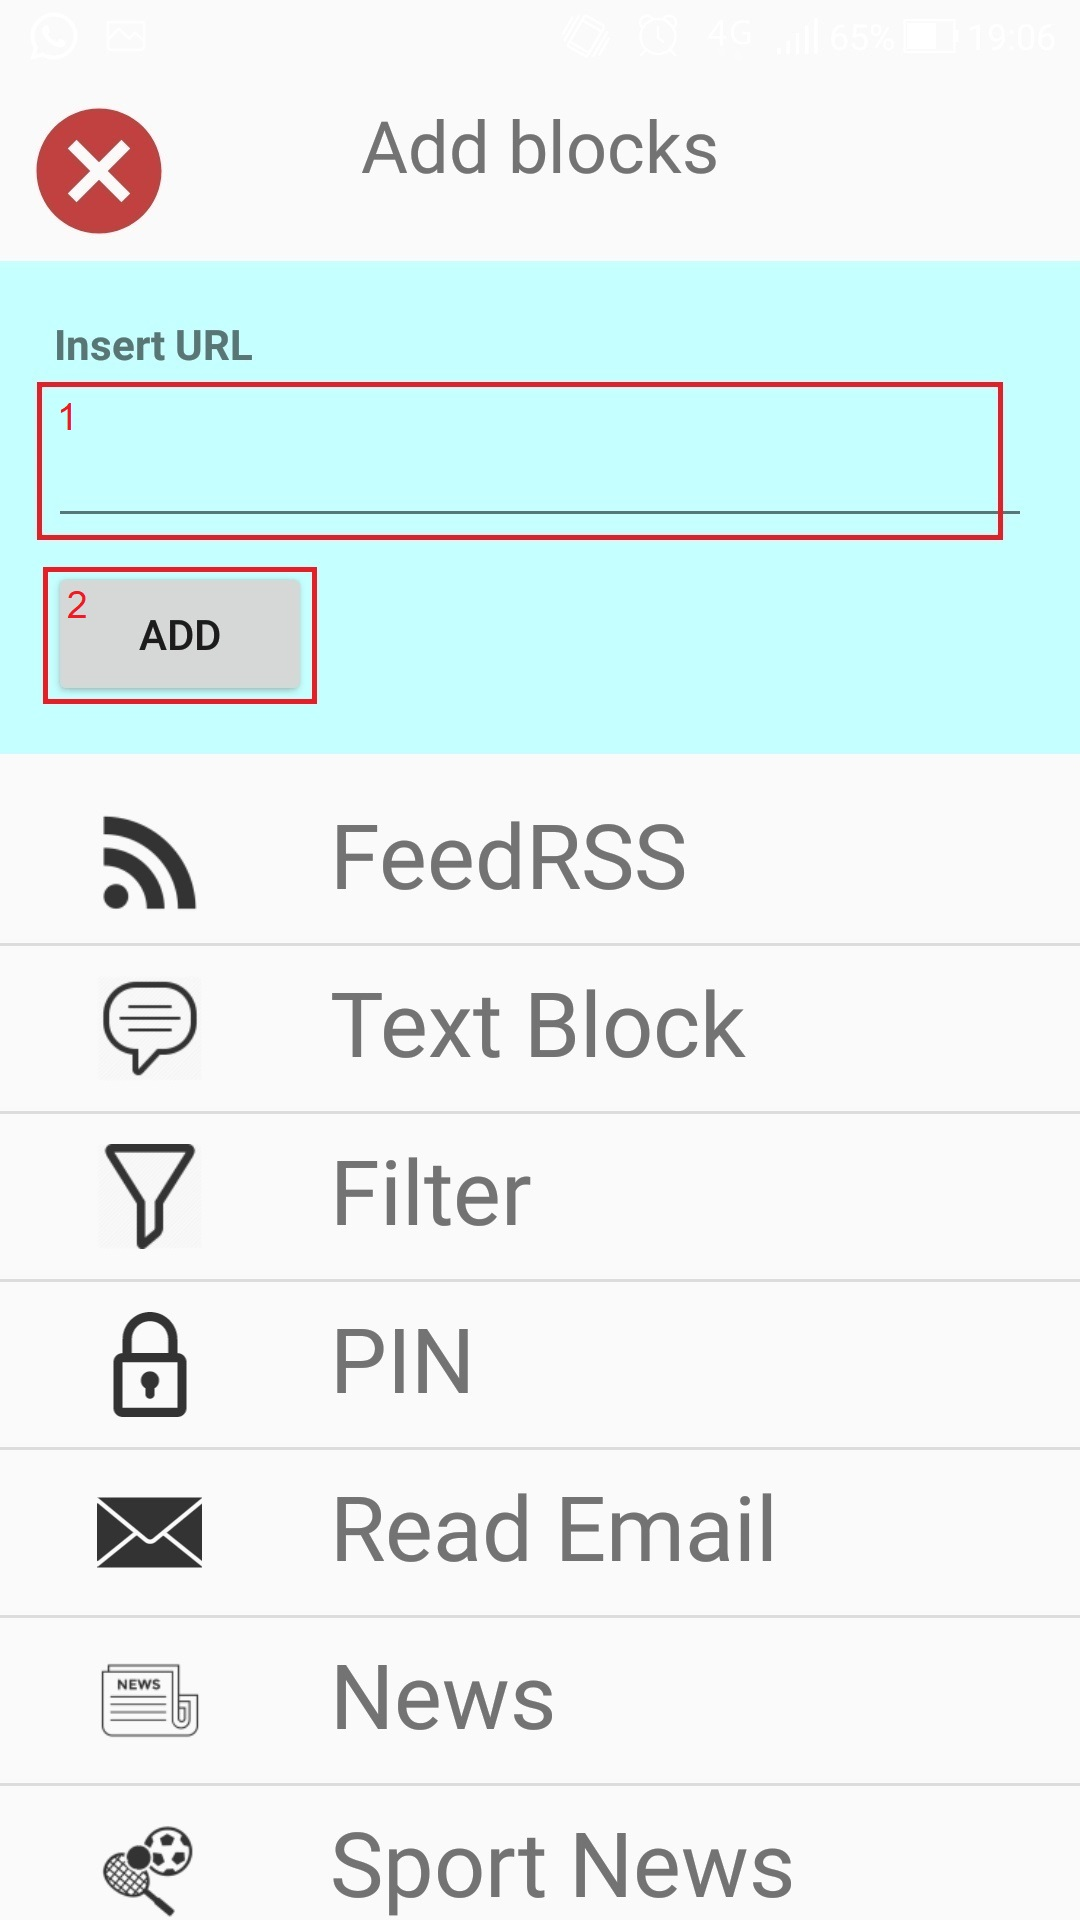
\includegraphics[scale=0.2]{images/BlockFeedRSS.jpg}}
	\caption{Blocco FeedRSS}
\end{figure}
\end{enumerate}
\newpage

\subsubsection{Blocco di testo}
Tale blocco consente all'utente di inserire nel proprio workflow un blocco contenente del testo.
\begin{enumerate}
	\item Inserire nell'apposito campo di input un testo a piacere;
	\item Confermare e salvare cliccando sul pulsante "ADD" per aggiungere il blocco al workflow.
	\begin{figure}[!ht]
		\centering
		\fbox{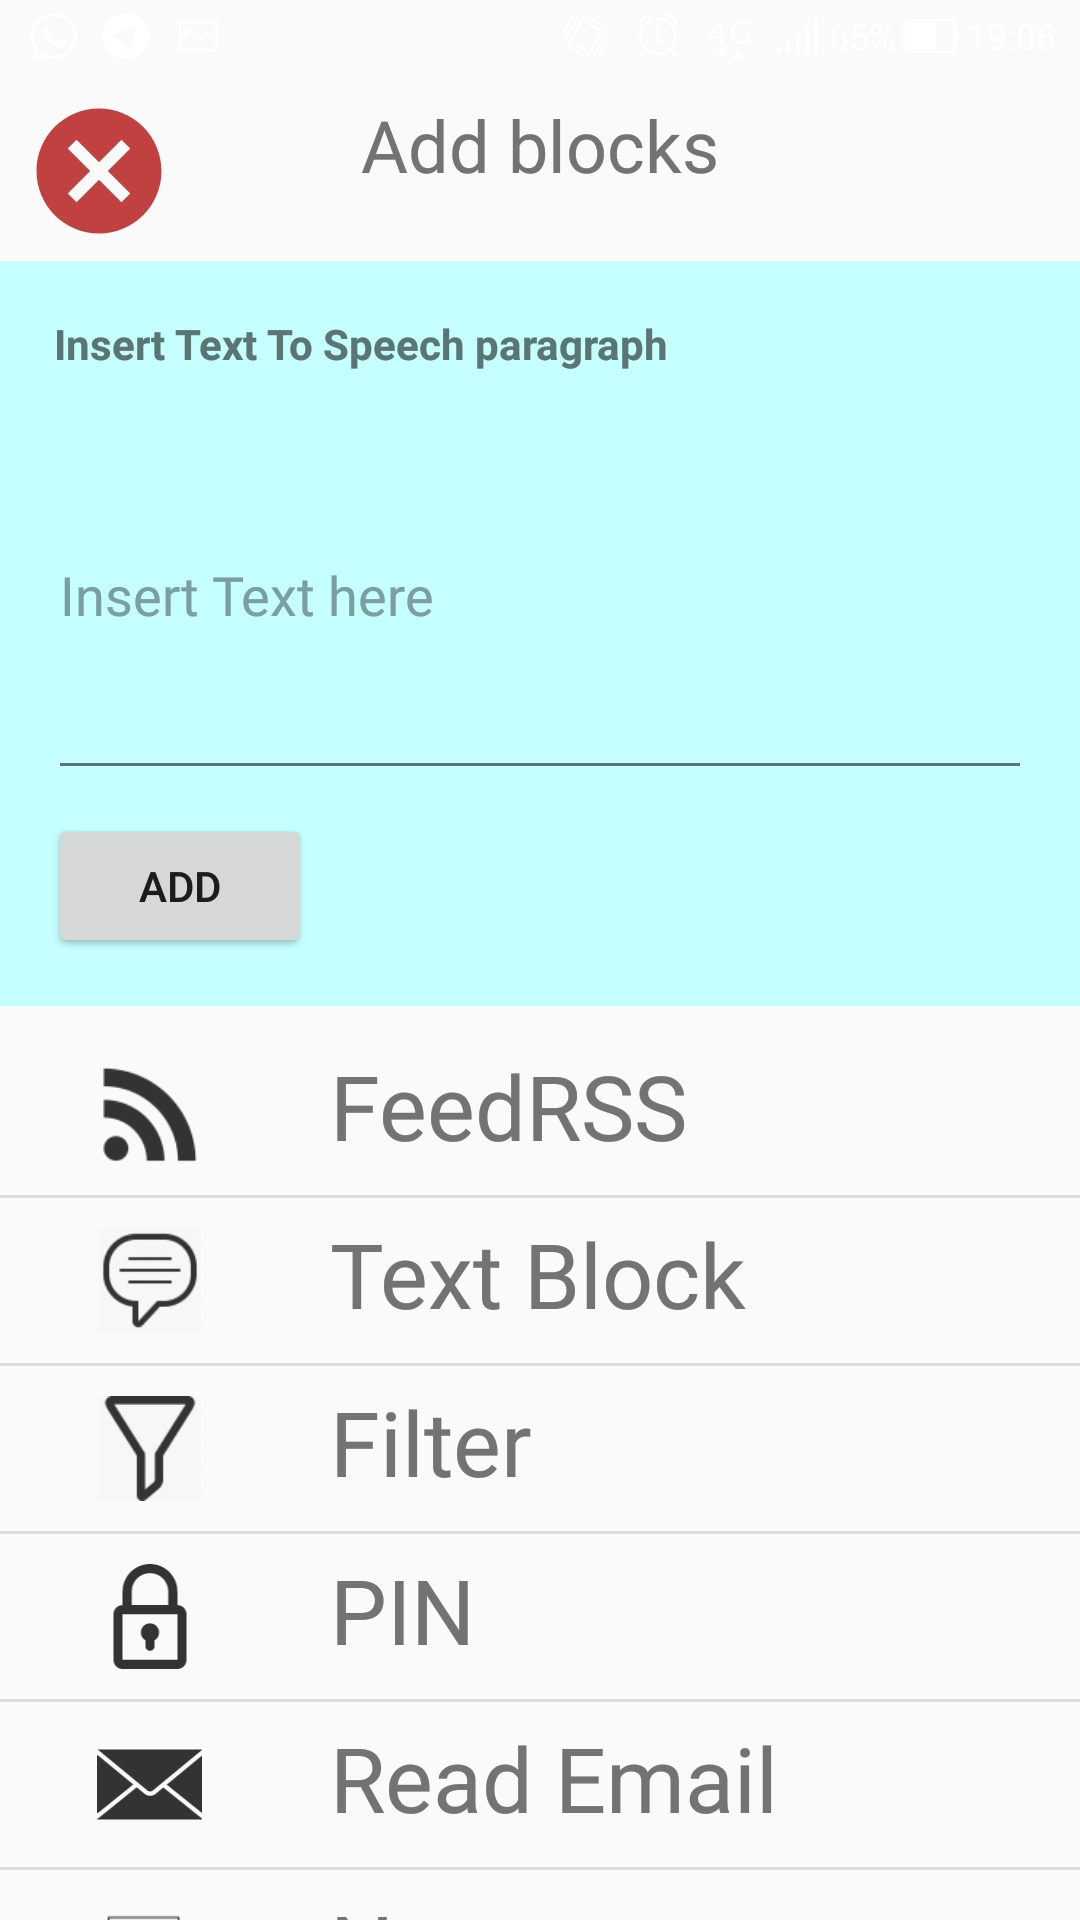
\includegraphics[scale=0.2]{images/BlockTextToSpeech.jpg}}
		\caption{Blocco di testo}
	\end{figure}
\end{enumerate}

\subsubsection{Blocco Filter}
Consente di impostare il numero limite di elementi che un determinato blocco deve considerare. \\
\textbf{NOTA BENE:} il blocco filtro è applicabile solo ai seguenti blocchi: Stock, Crypto, FeedRSS, News, Read Email, TwitterUserTimeline, TwitterHashtag, List e Sport.

\subsubsection{Blocco PIN}
Lo scopo di questo blocco è quello di effettuare una sorta di autenticazione dell'utente per l'esecuzione di alcuni blocchi, come ad esempio ReadEmail e Twitter in modo da avere un minimo di privacy per l'utente.
\begin{enumerate}
	\item Inserire nel campo di testo il proprio PIN segreto;
	\item Cliccare sul tasto "SAVE" per confermare e salvare.

	\begin{figure}[!ht]
		\centering
		\fbox{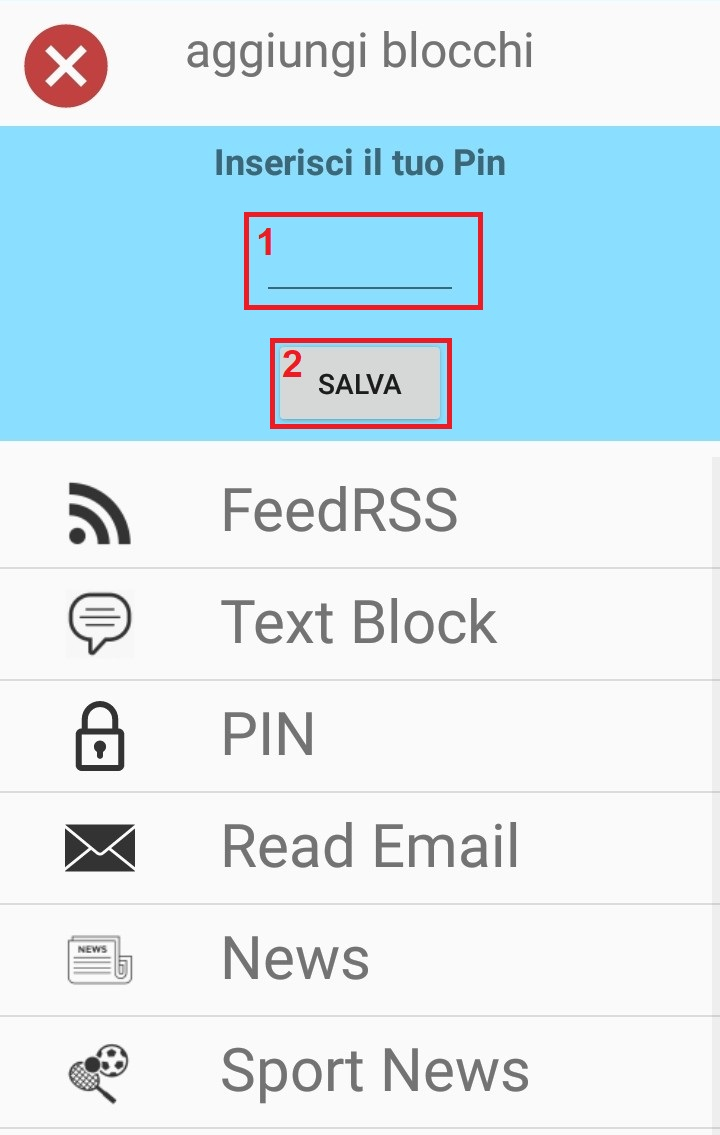
\includegraphics[scale=0.3]{images/BlockPIN.jpg}}
		\caption{Blocco PIN}
	\end{figure}
\end{enumerate}
\newpage
\subsubsection{Blocco News}
Tale blocco consente all'utente di ascoltare le ultime news prese da un sito a scelta tra i seguenti: Sky, Google News, Ansa, BBC, CNBC e Wall Street.
\begin{enumerate}
	\item Cliccare su un tasto a piacere tra quelli elencati per scegliere il sito da cui ricevere news.
	\begin{figure}[!ht]
		\centering
		\fbox{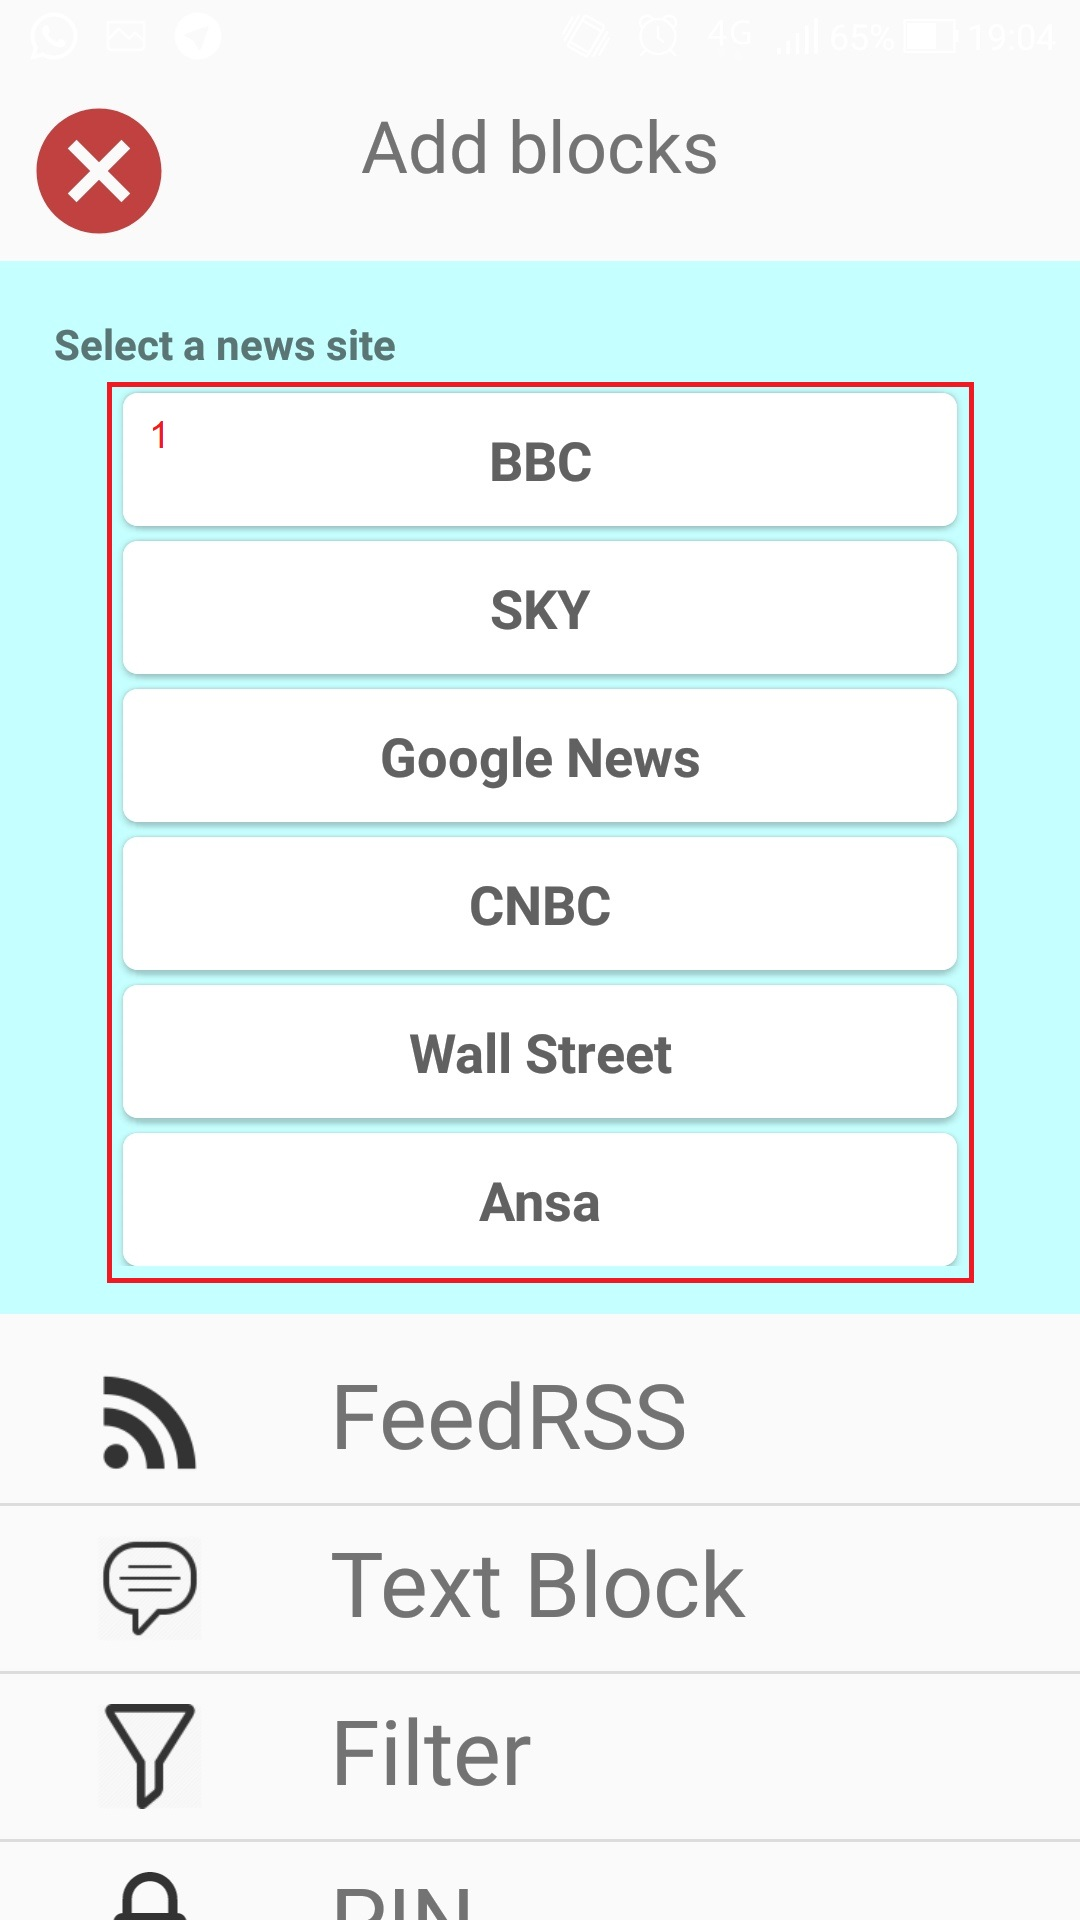
\includegraphics[scale=0.2]{images/BlockNews.jpg}}
		\caption{Blocco News}
	\end{figure}
\end{enumerate}
\newpage

\subsubsection{Blocco Sport}
Con l'aggiunta di questo blocco l'utente potrà ascoltare le ultime news riguardanti uno sport a sua scelta tra i seguenti: tennis, calcio, basket americano, formula1, football americano e motogp.
\begin{enumerate}
	\item Cliccare su un tasto a piacere tra quelli proposti per scegliere il sito da cui ricevere news sullo sport.
	\begin{figure}[!ht]
		\centering
		\fbox{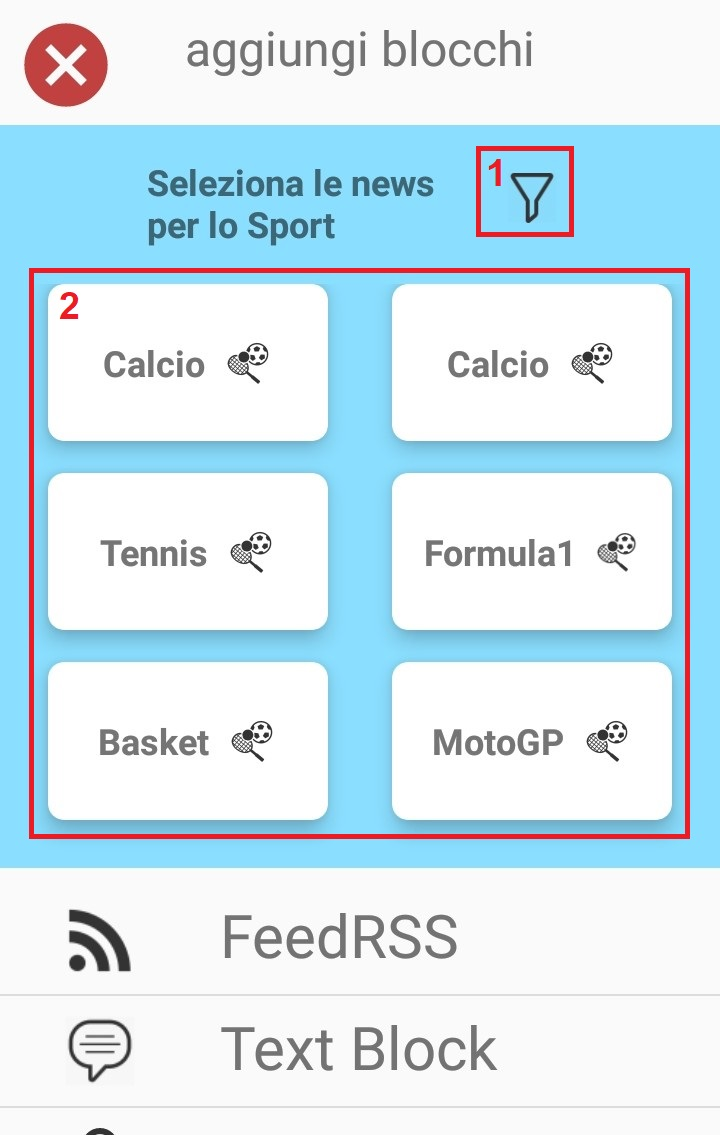
\includegraphics[scale=0.2]{images/BlockSport.jpg}}
		\caption{Blocco sport}
	\end{figure}
\end{enumerate}
\newpage
\subsubsection{Blocco Crypto}
Con questo blocco l'utente può scegliere da quale FeedRSS ascoltare le ultime news sulle cryptovalute.
\begin{enumerate}
	\item Cliccare su un tasto a piacere tra quelli proposti per scegliere da quale FeedRSS ricevere news sulle cryptovalute.
\begin{figure}[!ht]
	\centering
	\fbox{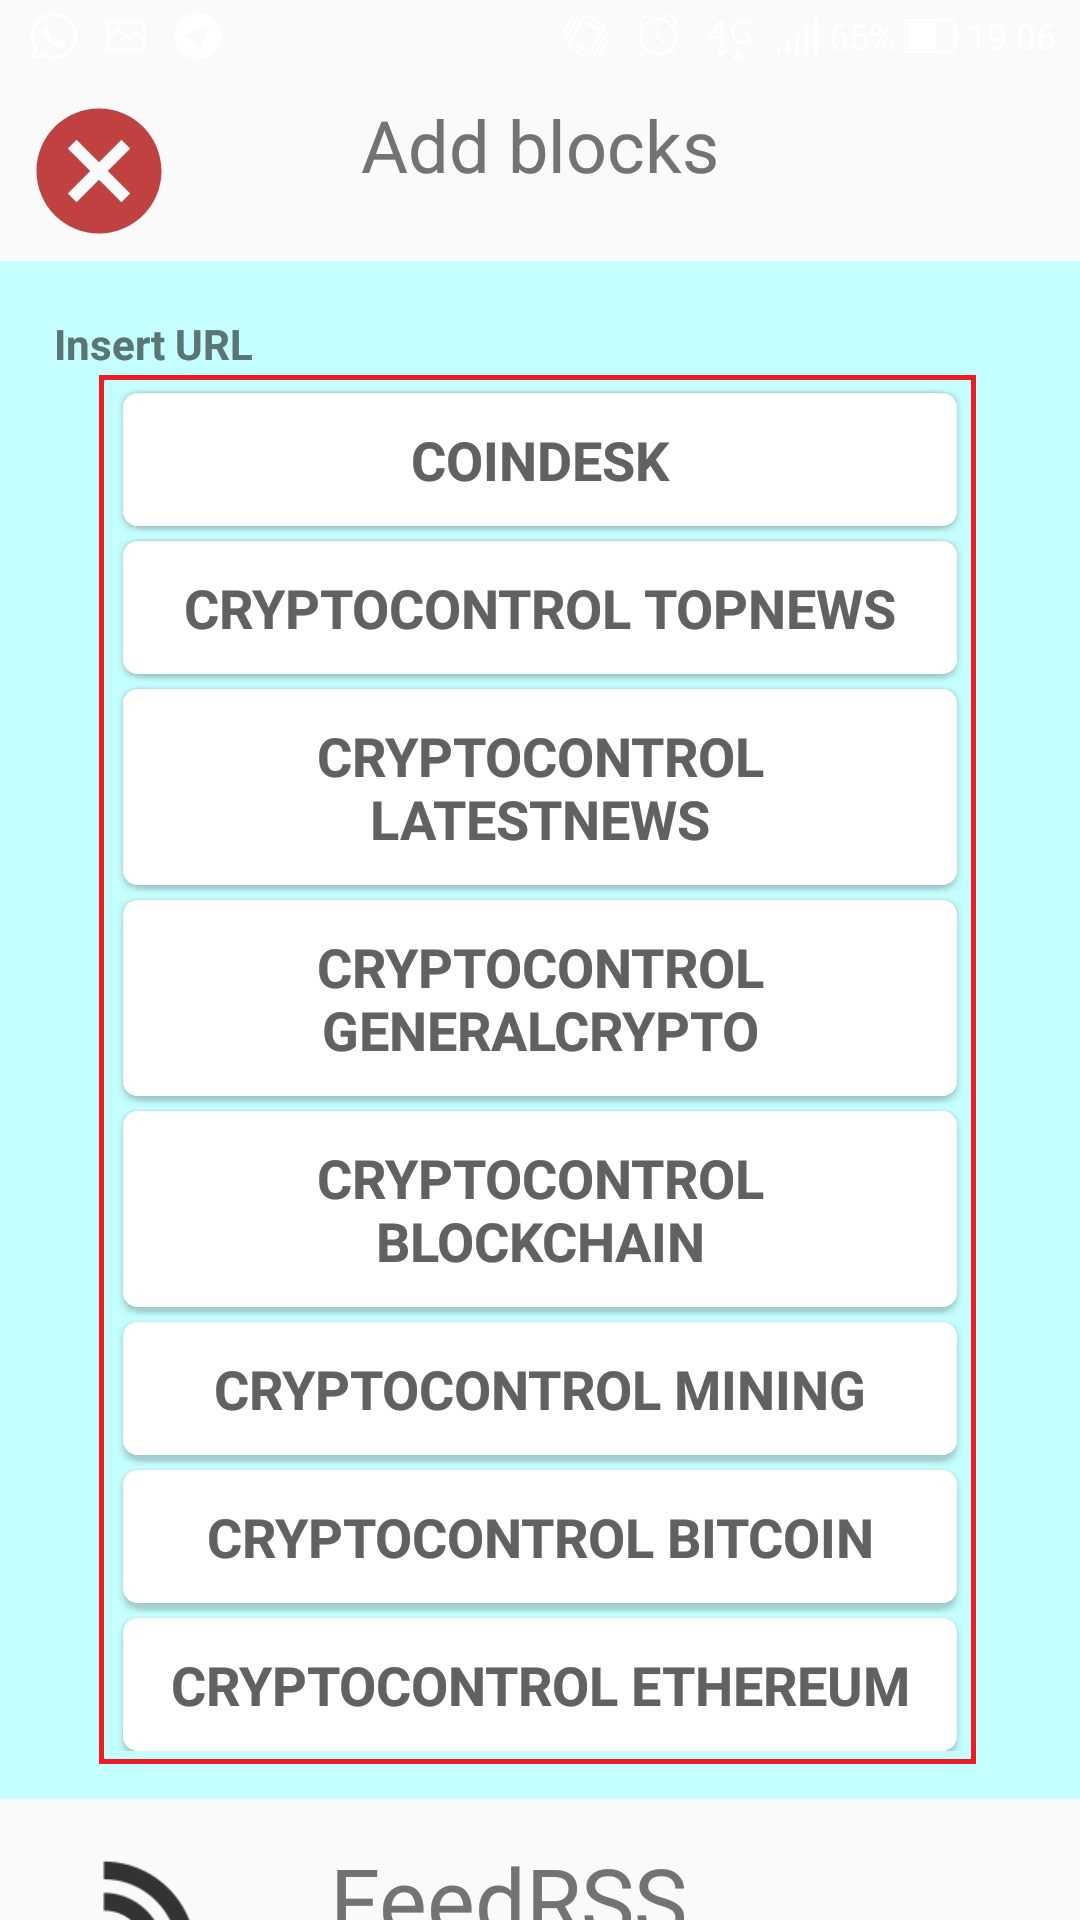
\includegraphics[scale=0.2]{images/BlockCrypto.jpg}}
	\caption{Blocco crypto}
\end{figure}
\end{enumerate}
\newpage
\subsubsection{Blocco Stock}
Con questo blocco l'utente può scegliere da quale FeedRSS ascoltare le ultime news sull'andamento della borsa economica.
\begin{enumerate}
	\item Cliccare su un FeedRSS a scelta per scegliere da quale borsa ricevere news.
\begin{figure}[!ht]
	\centering
	\fbox{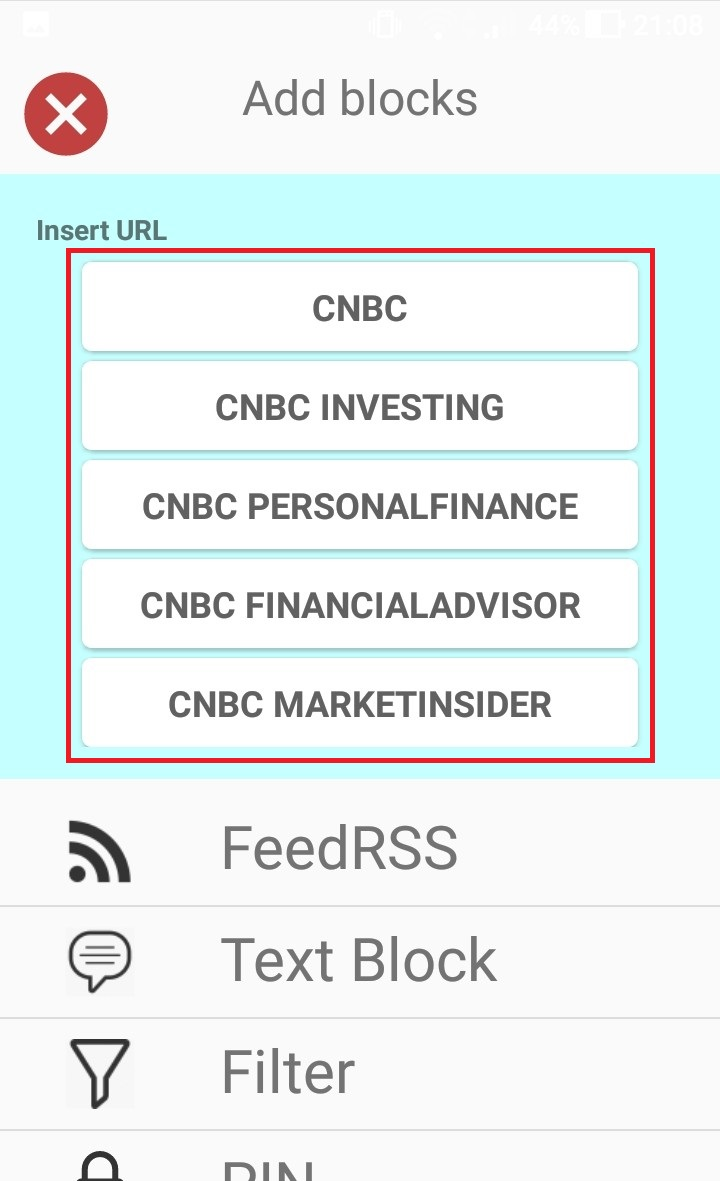
\includegraphics[scale=0.3]{images/BlockStock.jpg}}
	\caption{Blocco stock}
\end{figure}
\end{enumerate}
\newpage
\subsubsection{Blocco List}
Questo blocco permette all'utente di creare, aggiungere e modificare degli elementi di testo ad una lista.
È possibile modificare la lista tramite app oppure tramite interazione con l'Amazon Echo.

\subsubsection{Blocco TwitterHashtag}
L'utente con l'aggiunta di questo blocco può effettuare una ricerca su Twitter tramite hashtag.
\subsubsection{Blocco TwitterUserTimeline}
L'utente inserendo questo blocco nel suo workflow potrà sapere suoi i tweet.
\subsubsection{Blocco Weather}
Il blocco Weather consente all'utente di sapere che meteo c'è in questo momento o nei prossimi giorni di una determinata città.
\newpage
\subsection{Blocchi nel workflow}
Per avere informazioni sui blocchi contenuti in un workflow, andare sulla schermata che mostra l'elenco di tutti i workflow disponibili  e cliccare sul nome del workflow che ci interessa.
In questo modo verrà visualizzato l'elenco dei blocchi al suo interno come mostrato nella seguente figura:
\begin{figure}[!ht]
	\centering
	\fbox{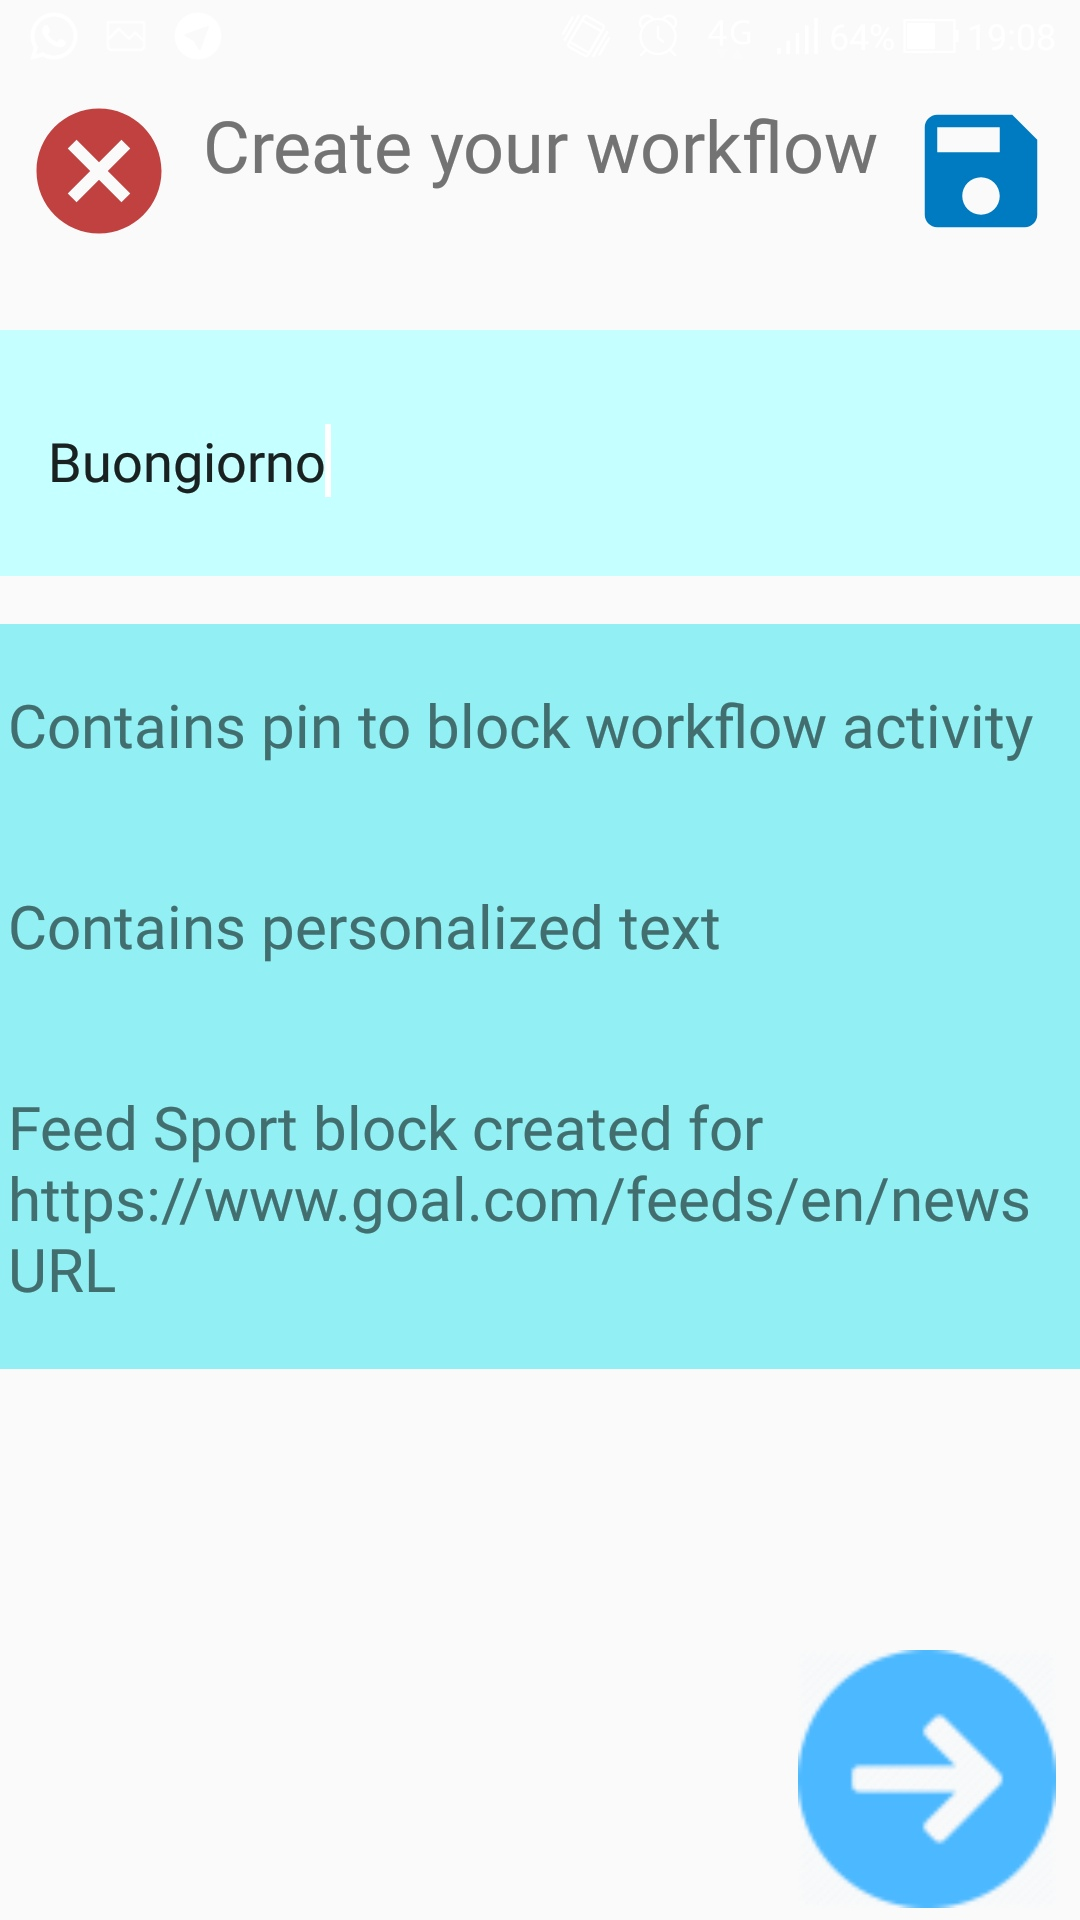
\includegraphics[scale=0.2]{images/BlocksWorkflow.jpg}}
	\caption{Blocchi del workflow}
\end{figure}
\newpage
\subsection{Modifica blocchi}
\subsection{Eliminazione blocchi}
\subsection{Eliminazione workflow}
\begin{comment}
\subsubsection{Blocco Amazon Music}
Questo blocco consente all'utente di ascoltare un brano, un'album o una playlist da Amazon Music tramite il proprio dispositivo Alexa.

\subsubsection{Blocco Telegram}
Il blocco Telegram consente all'utente iscritto al servizio di messaggistica Telegram di inviare messaggi e file audio ad un'altra persona o gruppo di persone.

\subsubsection{Blocco ReadEmail}
Con questo blocco l'utente può ascoltare tramite Alexa le sue email, di Gmail, non ancora lette.


\subsubsection{Blocco Calendar}
Il blocco calendario permette all'utente di ascoltare o aggiungere i suoi appuntamenti di Google calendar tramite l'Amazon echo.
\end{comment}
\newpage
\section{Utilizzo della skill MegAlexa}
\label{Utilizzo skill}
\begin{itemize}
\item  \textbf{Configurazione skill MegAlexa}\\
\label{Configurazione MegAlexa}
Per poter utilizzare la skill MegAlexa è necessario configurare il proprio account Amazon con la skill  attraverso l'applicazione Amazon Alexa installata sul dispositivo mobile. Per fare ciò seguire i seguenti passi:
\begin{enumerate}
	\item  Cliccare sulla voce "Skill e giochi"  presente nella barra laterale nell'applicazione Amazon Alexa ;
	
	\begin{figure}[!ht]
		\centering
		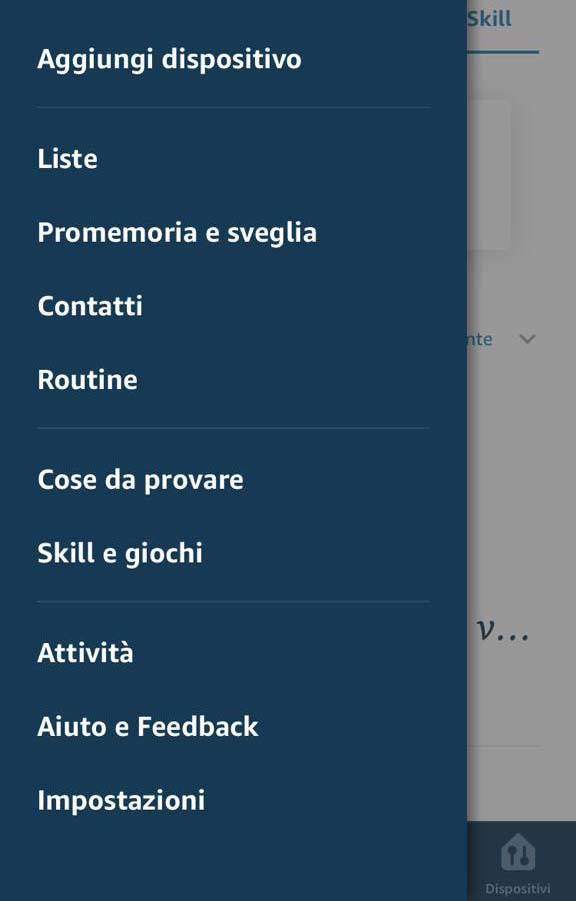
\includegraphics[width=0.5\textwidth]{images/SkillGiochi.png}
		\caption{Sezione skill e giochi di Amazon Alexa}
	\end{figure}
\newpage
	
	\item Andare sul simbolo delle lente di ingrandimento che indica la funzione di ricerca;
	\begin{figure}[H]
		\centering
		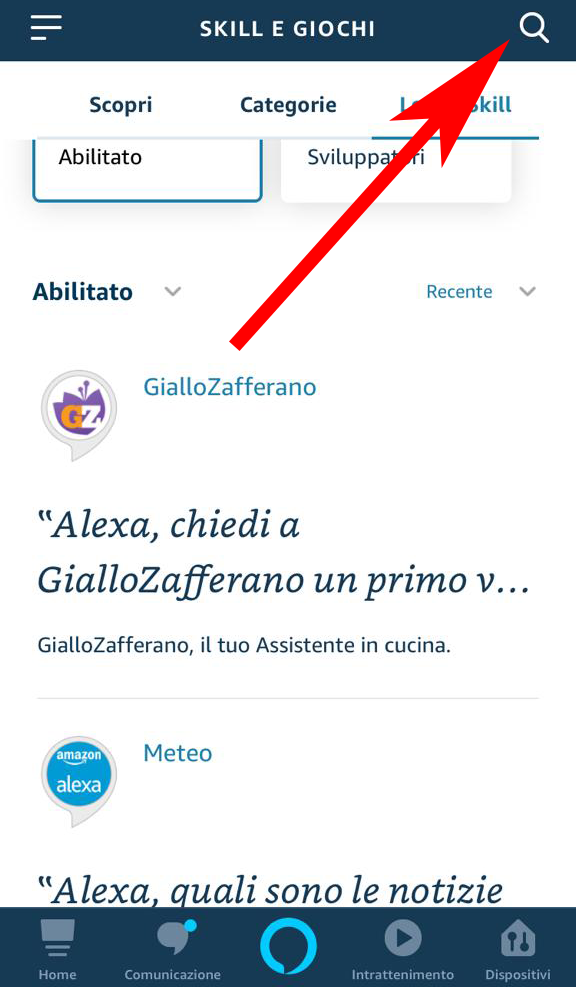
\includegraphics[width=0.5\textwidth]{images/SimboloCerca.png}
		\caption{Cerca di Amazon Alexa}
	\end{figure}
	\item Inserire il nome della skill che si sta cercando;
	\begin{figure}[!ht]
	\centering
	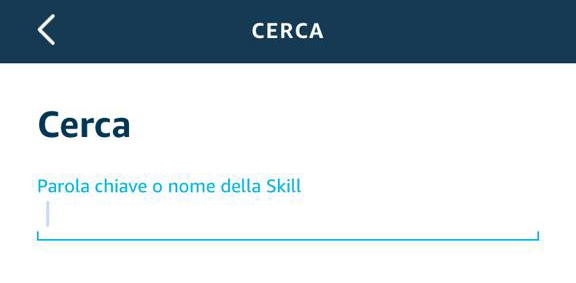
\includegraphics[width=0.5\textwidth]{images/CercaSkill.png}
	\caption{Inserimento nome Skill}
   \end{figure}
\newpage
    \item Abilitare la skill premendo il pulsante "Abilita all'uso";
    
    \begin{figure}[H]
    	\centering
    	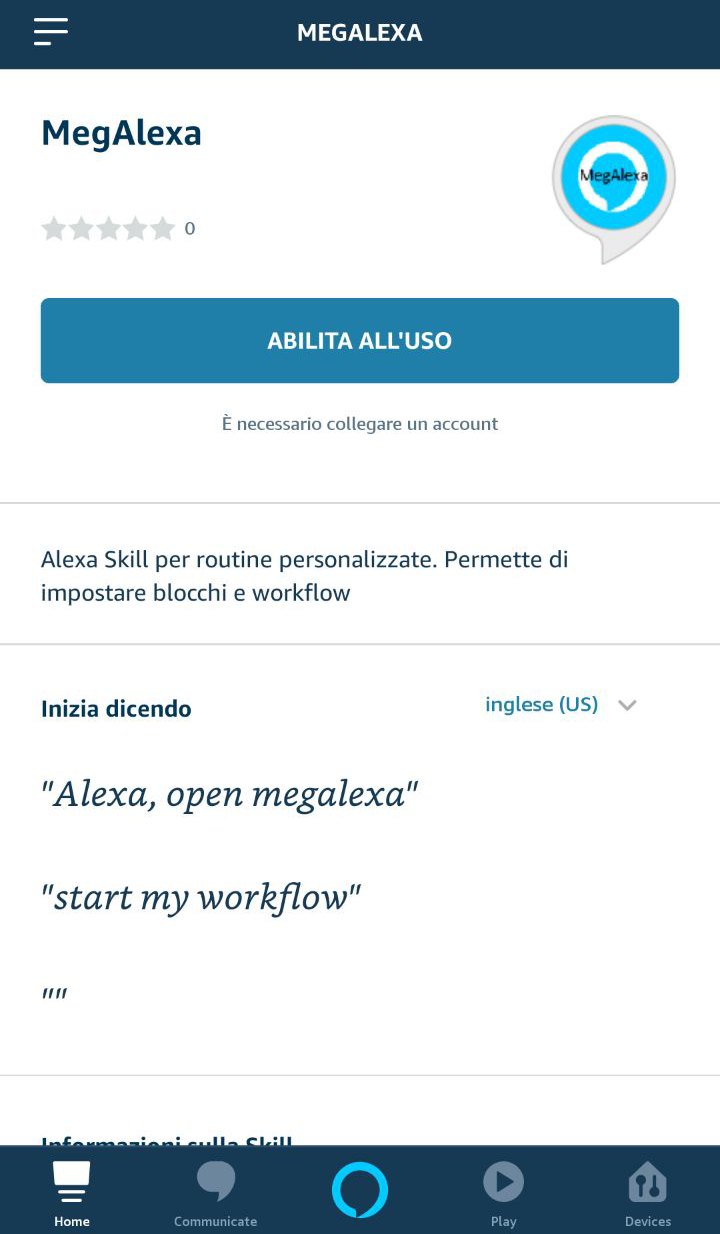
\includegraphics[width=0.5\textwidth]{images/AbilitaSkill.png}
    	\caption{Abilitazione Skill nell'applicazione Amazon Alexa}
    \end{figure}
    \newpage
    \item Collegare l'account Amazon con la Skill: dopo aver eseguito il punto numero 4, si verrà reindirizzati a una pagina di login di Amazon nella quale si dovranno inserire i dati relativi all'account Amazon che è in uso; \\
    
        \begin{figure}[H]
    	\centering
    	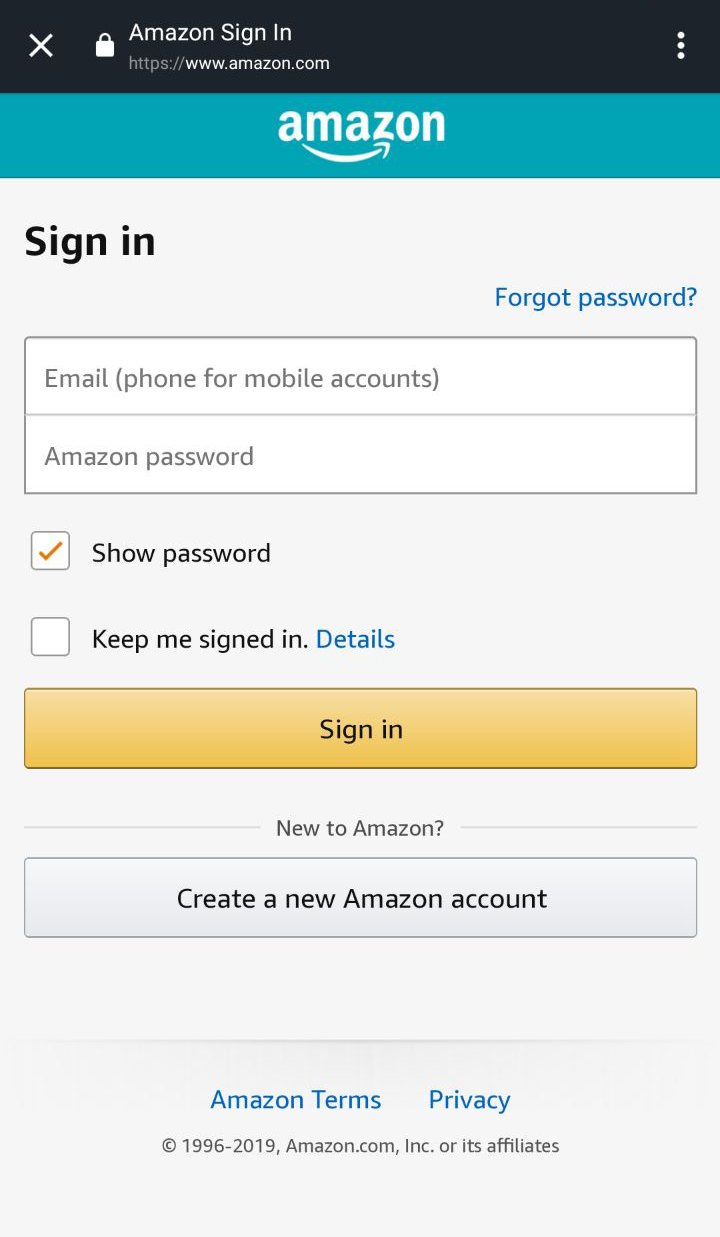
\includegraphics[width=0.5\textwidth]{images/AutenticazioneAccount.png}
    	\caption{Autenticazione Account Amazon}
    \end{figure}

    \newpage
     \item Skill collegata con successo;
     
       \begin{figure}[H]
     	\centering
     	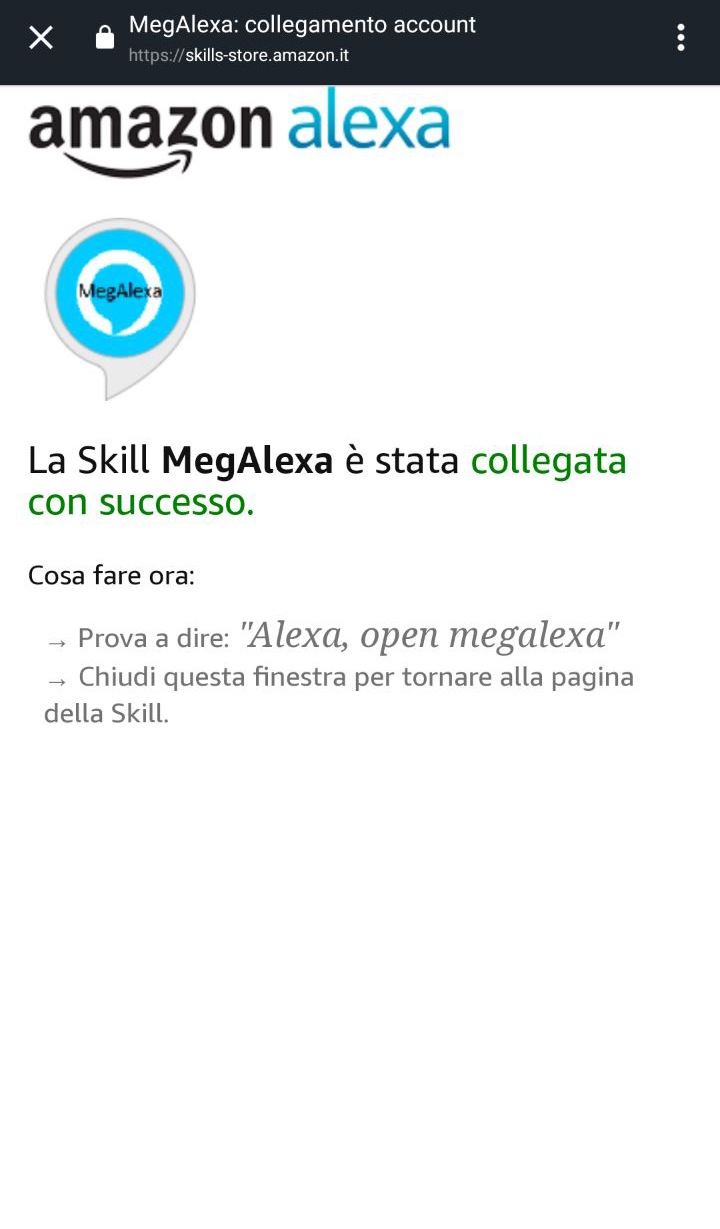
\includegraphics[width=0.5\textwidth]{images/AutenticazioneEseguita.png}
     	\caption{Collegamento Skill con successo}
     \end{figure}
    
    
    Ora il proprio account Amazon è collegato con la skill MegAlexa e si può procedere con l'esecuzione della skill
    attraverso l'iterazione vocale utilizzando l'Echo Dot.
    
\end{enumerate}
\newpage
\item  \textbf{Esecuzione skill MegAlexa}\label{Esecuzione skill}

Per avviare la skill MegAlexa attraverso l'Echo Dot occorre pronunciare uno dei comandi vocali di avvio come ad esempio: "Alexa, open MegAlexa", oppure "Alexa, start MegAlexa".
      
Se Alexa risponde con una richiesta dei configurazione dell'account Amazon con la skill MegAlexa allora  bisogna seguire le istruzioni indicate nella sezione precedente
\S\ref{Configurazione MegAlexa} "Configurazione Skill MegAlexa". 

\begin{figure}[!ht]
	\centering
	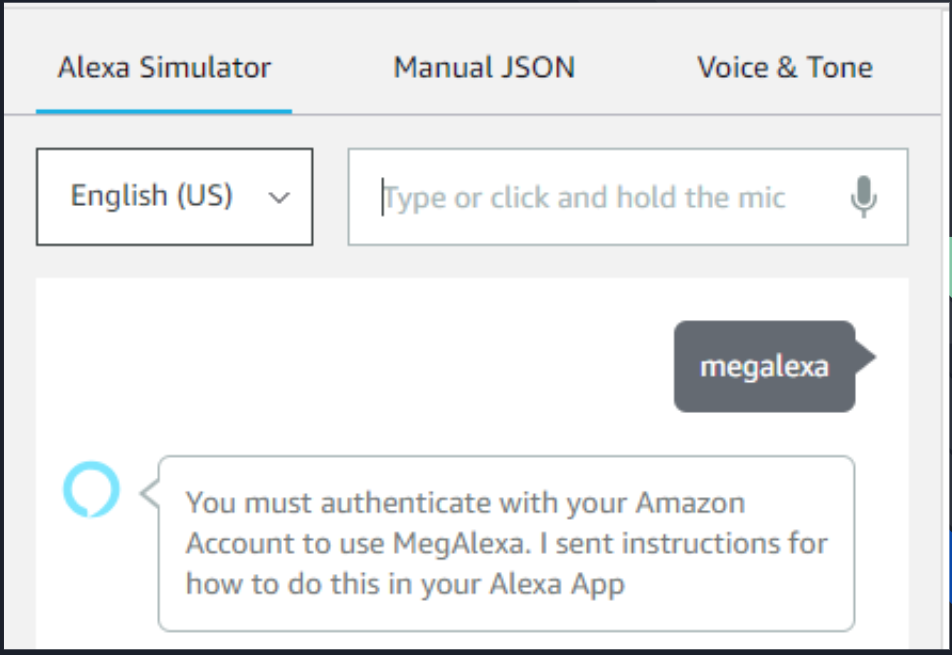
\includegraphics[width=0.5\textwidth]{images/RichiestaAutenticazione.png}
	\caption{Richiesta Autenticazione}
\end{figure}

Altrimenti si può procedere al successivo passaggio con l'esecuzione della skill MegAlexa attraverso l'iterazione vocale con Alexa. \\

\begin{figure}[!ht]
	\centering
	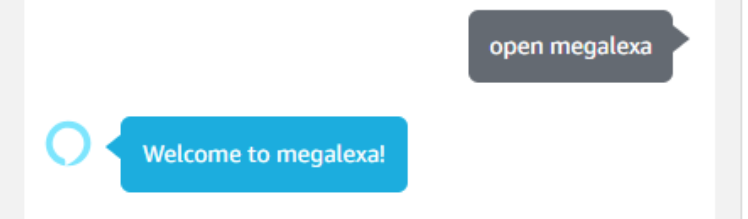
\includegraphics[width=0.5\textwidth]{images/OpenMegAlexa.png}
	\caption{Avvio della skill MegAlexa}
\end{figure}

\end{itemize}

A questo punto l'utente può avviare i workflow creati nell'applicazione.\\

\newpage
\section{Voice Dialog Flow}
\label{VDF}
Per riuscire a comprendere meglio come avviene l'interazione vocale con Alexa sono riportati dei Voice Dialog Flow, cioè degli esempi di conversazione.\\

Le interazioni sono strutturate come segue:
\begin{itemize}
	\item \textbf{U:} rappresenta l'utente;
	\item \textbf{A:} rappresenta Alexa;
	\item \textbf{[Data]:} rappresenta un dato il cui contenuto è determinato da risorse non presenti nel dispositivo al momento dell'interazione.
\end{itemize}

\subsection{Intents}
Per intent si intende la richiesta da parte dell'utente di effettuare una particolare operazione al fine di gestire l'esecuzione della\glossario{skill}. 
Questa sezione si occupa di elencare i principali intents a disposizione dell'utente, insieme agli output previsti una volta ricevuta la richiesta.
Si fa riferimento alla documentazione fornita da\glossario{Amazon}\footnote{\url{https://developer.amazon.com/it/documentation}} per lo sviluppo di una skill e la sua implementazione ottimale.

\subsection{Help Intent}\label{help}
Permette all'utente di ottenere ulteriori informazioni, come il numero di\glossario{workflow}disponibili e il loro contenuto.
\subsubsection{English}
\begin{itemize}
	\intent{help};
	\intent{help me};
	\intent{can you help me};
	\intent{tell me my workflows};
	\intent{i'd like a list of my workflows}.	
\end{itemize}
\subsubsection{Italiano}
\begin{itemize}
	\intent{aiuto};
	\intent{aiutami};
	\intent{aiuto per favore};
	\intent{dimmi i miei workflow};
	\intent{vorrei una lista dei miei workflow};
	\intent{quali sono i workflow disponibili?}.
\end{itemize}

\subsection{Cancel Intent}
Permette all'utente di cancellare un'azione in esecuzione (come l'avvio di un \textit{workflow$_{G}$}).
\subsubsection{English}
\begin{itemize}
	\intent{cancel};
	\intent{never mind};
	\intent{forget it}.
\end{itemize}

\subsubsection{Italiano}
\begin{itemize}
	\intent{annulla};
	\intent{non importa};
	\intent{lascia stare}.
\end{itemize}

\subsection{Stop Intent}
Permette all'utente di uscire dalla \textit{skill$_{G}$}.
\subsubsection{English}
\begin{itemize}	
	\intent{stop};
	\intent{off};
	\intent{shut up}.
\end{itemize}

\subsubsection{Italiano}

\begin{itemize}
	\intent{ferma};
	\intent{smettila};
	\intent{basta};
	\intent{stop};
	\intent{spegni}.
\end{itemize}


\subsection{Next Intent}
Consente di passare a un blocco successivo di un \textit{workflow$_{G}$}, sia nel caso in cui esso sia ancora in esecuzione oppure abbia terminato le proprie operazioni. 
\subsubsection{English}
\begin{itemize}
	\intent{next};
	\intent{skip};
	\intent{skip forward}.	
\end{itemize}

\subsubsection{Italiano}

\begin{itemize}
	
	\intent{prossimo};
	\intent{prossima};
	\intent{successivo};
	\intent{prosegui}.
	
\end{itemize}


\subsection{No Intent}
Consente all'utente di fornire una risposta negativa in seguito a una domanda di \textit{Alexa$_{G}$}.
\subsubsection{English}
\begin{itemize}
	
	\intent{no};
	\intent{no thanks};
	\intent{i'm good, thanks}.
	
\end{itemize}

\subsubsection{Italiano}
\begin{itemize}	
	\intent{no};
	\intent{no grazie};
	\intent{no basta così}.
	
\end{itemize}



\subsection{Pause Intent}
Permette di fermare temporaneamente l'esecuzione di un blocco all'interno di un \textit{workflow$_{G}$}.
\subsubsection{English}
\begin{itemize}
	
	\intent {pause};
	\intent {pause that}.
	
\end{itemize}

\subsubsection{Italiano}
\begin{itemize}
	
	\intent{metti in pausa};
	\intent{mettila in pausa}.
	
\end{itemize}


\subsection{Resume Intent}
Premette di riprendere l'esecuzione di un blocco all'interno di un\glossario{workflow}precedentemente fermato.
\subsubsection{English}
\begin{itemize}
	
	\intent{resume};
	\intent{continue};
	\intent{keep going}.
	
\end{itemize}

\subsubsection{Italiano}
\begin{itemize}
	\intent{riprendi};
	\intent{continua};
	\intent{riprendilo}.
	
\end{itemize}



\subsection{Yes Intent}
Consente all'utente di fornire una risposta positiva in seguito a una domanda di \textit{Alexa$_{G}$}.
\subsubsection{English}
\begin{itemize}
	
	\intent{yes};
	\intent{yes please};
	\intent{sure}.
	
\end{itemize}

\subsubsection{Italiano}
\begin{itemize}
	\intent{sì};
	\intent{sì per favore};
	\intent{certo};
	\intent{ok, va bene}.		
\end{itemize}

\subsection{Utilizzo blocco testo}
Al fine di creare workflow con blocchi che si collegano meglio tra di loro o per renderli più personalizzati,
nelle conversazioni che presentiamo molte delle frasi che Alexa andrà a dire costituiranno un blocco di testo, cioè un pezzo di testo che l'utente andrà a inserire prima dell'esecuzione di un blocco.

\subsection{English}
\subsubsection{Skill start} \label{SkillStart}
\textit{U: Open MegAlexa | Launch MegAlexa | Initiate MegAlexa | Start MegAlexa | Use MegAlexa | Begin MegAlexa}\\
\textbf{A: Welcome to MegAlexa, how can I help you? | Which workflow would you like to open?}

\subsubsection{Workflow start}
\textit{U: Open [workflow] | Initiate [workflow] | Start [workflow] | Use [workflow]}\\
With this interaction Alexa will start the workflow. \\
\textit{U: Show me my workflows | Tell me my workflows | Say my workflows}\\
\texttt{A: Your workflows are [workflow]}\\
\textit{U: Open [workflow] | Initiate [workflow] | Start [workflow] | Use [workflow]}

\begin{comment}
\texttt{A: Your workflows are [workflow]x3, do you want to hear more?}\\
\textit{U: [Yes Intent]}\\
\texttt{A: [workflow]x3, do you want to hear more?}\\
\textit{U: [No Intent], launch [workflow] | [No Intent], open [workflow] | [No Intent], initiate [workflow] | [No Intent], start [workflow] | [No Intent], use [workflow]}\\
If there are 3 or less workflows available, then Alexa won't ask to hear more workflows.\\
\texttt{A: Your workflows are [workflow]x2, which one would you like to start? }\\
\textit{U: Open [workflow] | Initiate [workflow] | Start [workflow] | Use [workflow]}
\end{comment}

\subsubsection{Workflow execution}

\subsubsection{Text to speech}
\texttt{A: [Text]}

\subsubsection{PIN}
\texttt{A: Say your pin to continue | What's your PIN? | Tell me your secret code | Let me know your PIN to continue | Confess me your secret code | Whisper your four digits number}\\
\textit{U: [PIN] }\\
If the user says the wrong PIN:\\
\texttt{A: Incorrect,please repeat | Wrong, try again | Wrong, retry }\\
\textit{U: [PIN]}\\\\
If the user says the correct PIN:\\
\texttt{A: PIN is correct.}\\


\subsubsection{Read Twitter}
\texttt{A: Those are your tweets: [Read tweets]}\\


\begin{comment}
QUESTA PARTE VA A DINDO
\subsubsection{Read Twitter}
\texttt{A: [Read tweets], do you want to hear more? | [Read tweets], should I keep reading? | [Read tweets], should I go on?}\\
\textit{U: [Yes Intent]}\\
\texttt{A: [Read tweets], do you want to hear more? | [Read tweets], should I keep reading? | [Read tweets], should I go on?}\\
\textit{U: [No Intent]}\\
\texttt{A: Ok | Alright}\\\\
If the user wish to continue listening tweets then Alexa will go forward reading the same amount of tweets set in the filterable block, otherwise Alexa will proceed with the next block.
\end{comment}

\subsubsection{Read List}
\texttt{A: Here are the element that you have in your list: [elements] | The items on your list are these: [elements] | Your list has these elements: [elements]}\\

\begin{comment}

\begin{itemize}
	\item The list is empty.\\
	\begin{itemize}
		//QUESTA PARTE VA A DINDO 
		\item Add an element on the list.\\
		\texttt{A: Your list is empty,add an element on the list | What element do you want to add?| Your list is blank, is there anything you want to fill it with?}\\
		\textit{U: Add [element] to my list | I'd like to insert [element] to my list | I want to add [element] to my list | I need to add [element] to my list | Add [element] }\\
		\texttt{A: Saved, would you like to add other elements? | Alright, would you like to add other elements? | Well done, do you have anything else to add? | Finally something in it, let's add some more}\\
		\textit{U: [No Intent]}\\
		\texttt{A: Ok | Alright}
		
		// PARTE VECCHIA
		\texttt{A: Would you like to add any elements into your list? | Your list is empty, is there anything you want to fill it with? | The list is empty, shall we insert anything? | There is nothing on your list, would you like to add any elements into your list? | Your list is blank, is there anything you want to fill it with?}\\
		\textit{U: Add [element] to my list | I'd like to insert [element] to my list | I want to add [element] to my list | I need to add [element] to my list | Add [element] }\\
		\texttt{A: Saved, would you like to add other elements? | Alright, would you like to add other elements? | Well done, do you have anything else to add? | Finally something in it, let's add some more}\\
		\textit{U: [No Intent]}\\
		\texttt{A: Ok | Alright}
		

		
	\end{itemize}
    QUESTA PARTE VA A DINDO 
	\item The list is not empty.\\
	\begin{itemize}
		\item Add an element on the list.
		\texttt{A: Add an element on the list | What element do you want to add?}\\
		\textit{U: Add [element] to my list | I'd like to insert [element] to my list | I want to add [element] to my list | I need to add [element] to my list | Add [element] }\\
		\texttt{A: Saved, would you like to add other elements? | Alright, would you like to add other elements? | Well done, do you have anything else to add?}\\
		\textit{U: [No Intent]}\\
		\texttt{A: Ok | Alright}
		
       PARTE VECCHIA
		\texttt{A: You have [x] elements on your list, here are the five most recent: [element]x5, would you like to hear more, modify or delete one of those? | You have [x] elements on your list, the last five elements you added are: [element]x5, would you like to hear more, modify or delete one of those? | Your list has [x] elements, here are the five most recent: [element]x5, would you like to hear more, modify or delete one of those?}\\
		\textit{U: [Yes Intent], I want to hear more | [Yes Intent], tell me more | [Yes Intent], go on | [Yes Intent] keep reading }\\
		\texttt{A: [element]x5, would you like to hear more, modify or delete one of those?}\\
		\textit{U: [No Intent]}\\
		\texttt{A: Ok, would you like to add any elements into your list? | Alright, would you like to add any elements into your list? | Ok, shall we insert anything?}\\
		\textit{U: Add [element] to my list | I'd like to insert [element] to my list | I want to add [element] to my list | I need to add [element] to my list | Add [element] }\\
		\texttt{A: Saved, would you like to add other elements? | Alright, would you like to add other elements? | Well done, do you have anything else to add? | Ok, let's add some more}\\
		\textit{U: [No Intent]}\\
		\texttt{A: Ok | Alright}
		
		
		QUESTA PARTE VA A DINDO
		\item Change an element on the list.\\
		\texttt{A:Which element do you want to change?}
	    \textit{U: Change [old element]  | Edit [old element]]}\\
	    \texttt{A: What do you want to insert instead of the old element?}
	     \textit{U: [new element]}\\
	    \texttt{A: Ok, the change has been successfully applied, would you like to change others elements?| The edit has been successfully applied,would you like to change others elements?}\\
	     \textit{U: [No Intent] }\\
	    \texttt{A: Ok | Alright}
	    
	    
		PARTE VECCHIA
		\texttt{A: You have [x] elements on your list, here are the five most recent: [element]x5, would you like to hear more, modify or delete one of those? | You have [x] elements on your list, the last five elements you added are: [element]x5, would you like to hear more, modify or delete one of those? | Your list has [x] elements, here are the five most recent: [element]x5, would you like to hear more, modify or delete one of those?}\\
		\textit{U: Change [old element] with [new element] | Edit [old element] with [new element]}\\
		\texttt{A: The change has been successfully applied, would you like to change or delete anything else? | The edit has been successfully applied, would you like to change or delete anything else?}\\
		\textit{U: [Yes Intent], change [old element] with [new element] | edit [old element] with [new element]}\\
		\texttt{A: The change has been successfully applied, would you like to change or delete anything else? | The edit has been successfully applied, would you like to change or delete anything else?}\\
		\textit{U: [No Intent]}\\
		\texttt{A: Ok, would you like to hear others elements? | Alright, would you like to hear others elements? }\\
		\textit{U: [Yes Intent] }\\
		\texttt{A: [element]x5, would you like to hear more, modify or delete one of those?}\\
		\textit{U: [No Intent] }\\
		\texttt{A: Ok | Alright}

		
		QUESTA PARTE VA A DINDO
		\item Delete an element on the list.\\
		\texttt{A:Which element do you want to delete?}
		\textit{U: [element]}\\
		\texttt{A: Ok, The element has been successfully deleted, would you like to delete others elements? | Alright, would you like to delete anything else? | The element has been successfully dropped, would you like to delete others elements?}\\
		\textit{U: [No Intent]}\\
		\texttt{A: Ok}
		
		PARTE VECCHIA
		\texttt{A: You have [x] elements on your list, here are the five most recent: [element]x5, would you like to hear more, modify or delete one of those? | You have [x] elements on your list, the last five elements you added are: [element]x5, would you like to hear more, modify or delete one of those? | Your list has [x] elements, here are the five most recent: [element]x5, would you like to hear more, modify or delete one of those?}\\
		\textit{U: Delete [element] | Drop [element]}\\
		\texttt{A: The element has been successfully deleted, would you like to change or delete anything else? | The element has been successfully dropped, would you like to change or delete anything else?}\\
		\textit{U: [Yes Intent], delete [element] | [Yes Intent], drop [element]}\\
		\texttt{A: The element has been successfully deleted, would you like to change or delete anything else? | The element has been successfully dropped, would you like to change or delete anything else?}\\
		\textit{U: [No Intent]}\\
		\texttt{A: Ok, would you like to hear the other elements? | Alright, would you like to hear the other elements? }\\
		\textit{U: [Yes Intent] }\\
		\texttt{A: [element]x5, would you like to hear more, modify or delete one of those?}\\
		\textit{U: [No Intent]}\\
		\texttt{A: Ok | Alright}
		
     	QUESTA PARTE VA A DINDO
		\item Clear list.\\
	    \texttt{A: would you like to delete all the list? |  would you like to delete all the  elements?}
		\textit{U: Yes}\\
		\texttt{A: Ok, list deleted.}
		
		PARTE VECCHIA
		\texttt{A: You have [x] elements on your list, here are the five most recent: [element]x5, would you like to hear more, modify or delete one of those? | You have [x] elements on your list, the last five elements you added are: [element]x5, would you like to hear more, modify or delete one of those? | Your list has [x] elements, here are the five most recent: [element]x5, would you like to hear more, modify or delete one of those?}\\
		\textit{U: Clear my list}\\
		\texttt{A: Would you like to add any elements into your list? | Your list is empty, is there anything you want to fill it with? | The list is empty, shall we insert anything? | There is nothing on your list, would you like to add any elements into your list? | Your list is blank, is there anything you want to fill it with?}\\
		\textit{U: Add [element], and [element] to my list | I'd like to insert [element] to my list | I want to add [element] to my list | I need to add [element] to my list | Add [element], and [element] | Add [element]}\\
		\texttt{A: Saved, would you like to add other elements? | Alright, would you like to add other elements? | Well done, do you have anything else to add? | Ok, let's add some more}\\
		\textit{U: [No Intent]}\\
		\texttt{A: Ok | Alright}

	\end{itemize}
	
	If there are less then 6 elements, Alex won't ask the user to hear other elements.\\
	\texttt{A: You have [x] elements on your list: [element] would you like to modify or delete one of those? | You have [x] elements on your list: [element] would you like to modify or delete one of those? | Your list has [x] elements: [element] would you like to modify or delete one of those?}\\
	\textit{U: [No Intent]}	
		 \end{itemize}
		 
\end{comment}

	 

\begin{comment}
\subsubsection{Read email}
\begin{itemize}
	\item User has no unread emails\\
	\texttt{A: You haven't new emails | Wonderful, you already have read all your emails | Relax, you haven't receive new emails | Awesome, you haven't new emails}\\
	\textit{U: Ok | Alright}
	\item User has new emails to read\\
	\texttt{A: You have [x] new emails, would you like to read them? | There are [x] new emails, would you like to read them? }\\
	\textit{U: [Yes Intent]}\\
	\texttt{A: [emails], there are [x] emails left, would you like to continue reading? | [emails], would you like to continue reading [x] remaining emails? | [emails], there are [x] remaining emails, would you like to continue reading? | [emails], there are [x] emails left, should I keep reading? | [emails], should I keep reading [x] remaining emails?}\\
	\textit{U: [No Intent] }\\
	\texttt{A: Ok | Alright}
	
	If the user has new emails, Alexa will proceed to read them all. Also the user can choose a filter block which can allow him to read a selected amount of emails.
\end{itemize}

\subsubsection{Calendar}//NO
\begin{itemize}
	\item Read events
	\begin{itemize}
		\item There are no events to read.\\
		\texttt{A: You have no events today | Wonderful, there are no events today}\\
		\textit{U: Ok | Alright}
		\item There are events to read.\\
		\texttt{A: You have [x] events today, [events] | There are [x] scheduled for today, [events]}
	\end{itemize}
	\item Create events\\
	\texttt{A: When will be the event? | When would you like the event to be scheduled?}\\
	\textit{U: It will be for [time] | Set it for [time] | Create an event for [time]}\\
	\texttt{A: Which name the event has? | What is the event's name? | Tell me the name of the event | Which name should I set?}\\
	\textit{U: Set [name] | The name is [name] | Save event as [name]}\\
	\texttt{A: Alright, events is been successfully saved, would you like to add another event? | Event has been saved, would you like to add other events?}\\
	\textit{U: [No Intent]}
\end{itemize}
\end{comment}

\subsubsection{Feed RSS}
\texttt{A: Here is your feed, [FeedRSS]}

\subsubsection{Weather}
\texttt{A: Currently in [Location] is [$^\circ$C], with [Weather] you can expect an hight of [$^\circ$C] and a low of [$^\circ$C]}
\begin{comment}
\subsubsection{Amazon Music}//NO
\texttt{A: Let's listen to some good music, [playlist] | Let's play some music [playlist]}
\end{comment}

\subsubsection{News}
\texttt{A: Here is your flash briefing [news] | Here are the news [news]}

\subsubsection{Sport}
\texttt{A: Here is your sport flash briefing [sport]}

\subsubsection{Stock}  
\texttt{A: Here are your stock-market news [stock]}

\subsubsection{Crypto}   
\texttt{A: Here are your cryptocurrency related news [stock]}

\subsubsection{Workflow is done}
\texttt{A: Your workflow is completed, would you like to start a new one?}\\
At this point Alexa will wait the user's response and proceed with the Start Skill interaction described at \ref{SkillStart}.

\subsection{Italiano}
\subsubsection{Inizializzazione skill} \label{InizializzazioneSkill}
\textit{U: Apri MegAlexa | Lancia MegAlexa | Inizia MegAlexa | Usa MegAlexa | Esegui MegAlexa | Fai partire MegAlexa}\\
\textbf{A: Benvenuto in MegAlexa, come posso aiutarti? | Quale workflow desideri aprire? | Con quale workflow vuoi iniziare? | Da quale workflow partiamo?}

\subsubsection{Inizializzazione workflow}
\textit{U: Apri [workflow] | Inizia [workflow] | Usa [workflow] | Fai partire [workflow] | Esegui [workflow]}\\
Con questa interazione Alexa inizierà l'esecuzione del workflow.\\
\textit{U: Quali workflows ho a disposizione? | Quali sono i miei workflows? | Non mi ricordo i workflows, elencameli | Quali workflows posso eseguire? | Elencami i miei workflows | Quali workflows posso usare?}\\
\texttt{A: I tuoi workflows sono i seguenti [workflow]| Hai a disposizione i seguenti [workflow]}\\
\begin{comment}
\texttt{A: I tuoi workflows sono[workflow]x3, vuoi sentirne altri? | Puoi usare [workflow]x3, vuoi sentire i rimanenti?}\\
\textit{U: [Sì Intent]}\\
\texttt{A: I tuoi workflows sono, [workflow]x3, vuoi sentirne altri? | Puoi usare [workflow]x3, vuoi sentire i rimanenti?}\\
\textit{U: [No Intent], apri [workflow] | [No Intent], inizia [workflow] | [No Intent], usa [workflow] | [No Intent], fai partire [workflow] | [No Intent], esegui [workflow]}\\
Nel caso in cui ci fossero meno di 4 workflows allora Alexa non chiederà più di sentire i rimanenti workflows.\\
\texttt{A: I tuoi workflows sono [workflow]x2, quale vuoi scegliere?}\\
\textit{U: Apri [workflow] | Inizia [workflow] | Usa [workflow] | Fai partire [workflow] | Esegui [workflow]}\\
\end{comment}

\subsubsection{Esecuzione del workflow}

\subsubsection{Testo personalizzato}
\texttt{A: [Testo]}

\subsubsection{PIN}
\texttt{A: Qual è il tuo codice? | Dimmi il tuo codice segreto | Confessami il tuo codice per continuare | Qual è il tuo PIN? | Dimmi le quattro cifre segrete}\\
\textit{U: [PIN]}\\
\texttt{A: Sbagliato, riprova | Codice non corretto, riprova}\\
\textit{U: [PIN]}\\
Quando l'utente dirà il PIN corretto allora Alexa proseguirà con l'esecuzione del workflow.

\subsubsection{Lettore Twitter}
\texttt{A: Questi sono i tweet:[Legge tweets] | Ecco i tweet:[Legge tweets]}\\


\begin{comment}
\subsubsection{Lettore Twitter}
\texttt{A: [Legge tweets], vuoi ascoltarne altri? | [Legge tweets], vuoi sentirne altri? | [Legge tweets], ne leggo altri? | [Legge tweets], continuo a leggerne?}\\
\textit{U: [Sì Intent]}\\
\texttt{A: [Legge tweets], vuoi ascoltarne altri? | [Legge tweets], vuoi sentirne altri? | [Legge tweets], ne leggo altri? | [Legge tweets], continuo a leggerne?}\\
\textit{U: [No Intent]}\\
\texttt{A: Ok | Va bene}
\end{comment}

\subsubsection{Lettore Lista}
\texttt{A: Questi sono gli elementi nella lista:[elementi] | Ecco gli elementi nella lista:[elementi] | La tua lista contiene questi elementi: [elementi] }\\



\begin{comment}
\begin{itemize}
	\item La lista è vuota.\\
	\item Aggiungere un elemento alla lista.\\
	\texttt{A: Vuoi aggiungere un elemento alla tua lista vuota? | La lista  è vuota, vuoi aggiungere un elemento? | Aggiungi il primo elemento alla tua lista | La lista è vuota desideri aggiungere qualche elemento? | La lista è vuota, aggiungiamoci qualcosa }\\
	\textit{U: Aggiungi [elemento] alla mia lista | Aggiungi [elemento] alla lista | Vorrei aggiungere [elemento] | Aggiungi [elemento] | Voglio aggiungere [elemento] | Metti [elemento] dentro la lista | Metti [elemento] nella lista }\\
	\texttt{A: Elemento salvato, vuoi aggiungerne altri? | Elemento salvato con successo, vuoi aggiungere altro? | Elemento aggiunto alla lista, aggiungiamo altro? | Fatto, aggiungiamo altri elementi? | Aggiungiamo altri elementi? }\\
	\textit{U:[No Intent]}\\
	\texttt{A: Va bene | Ok }\\ 
	

	\item La lista non è vuota.\\
	\begin{itemize}
		PARTE VECCHIA
		\item Aggiungere un elemento alla lista.
		\texttt{A: Hai [x] elementi nella tua lista, questi sono i più recenti: [elemento]x5, vuoi che te ne legga altri oppure preferisci modificare o eliminare uno di questi? | Hai [x] elementi nella tua lista, gli ultimi che hai aggiunto sono: [elemento]x5, vuoi sentirne altri oppure vuoi modificare o eliminare uno di questi? | La tua lista ha [x] elementi, questi sono i più recenti: [elemento]x5, vuoi sentirne altri oppure modificare o eliminare uno di questi? }\\
		\textit{U: [Si Intent], voglio sentirne altri | [Si Intent], continua a leggere | [Si Intent], leggine altri | [Si Intent], continua con la lettura }\\
		
		NUOVA PARTE PER DINDO
		\texttt{A: Aggiungi un elemento alla lista}
		\textit{U: [elemento]}\\
       \texttt{A: Vuoi aggiungere un altro elemento?}
       	\textit{U: No]}\\
		
		\begin{comment}
		\texttt{A: [elemento]x5, vuoi sentirne altri oppure vuoi modificare o eliminare uno di questi? }\\
		\textit{U: [No Intent]}\\
		\texttt{A: Va bene, vuoi aggiungere un elemento alla tua lista? | Ok, vuoi aggiungere qualche elemento alla tua lista? | Ok, aggiungiamo qualche elemento? | Va bene, vuoi inserire qualcosa nella tua lista? }\\
		\textit{U: Aggiungi [elemento] alla mia lista | Vorrei aggiungere [elemento] alla mia lista | Aggiungi [elemento] | Inserisci [elemento] nella mia lista | Inserisci [elemento] nella lista  | Inserisci [elemento]}\\
		\texttt{A: Salvato con successo, vuoi aggiungere altri elementi? | Va bene, vuoi aggiungere altri elementi? | Salvato, vuoi aggiungerne altri? | Fatto, vuoi aggiungerne altri? }\\
		\textit{U: [No Intent]}\\
		\texttt{A: Va bene | Ok}
		
		PARTE VECCHIA
		\item Modifica di un elemento nella lista.\\
		 \begin{comment}
		 \texttt{A: Hai [x] elementi nella tua lista, questi sono i più recenti: [elemento]x5, vuoi che te ne legga altri oppure preferisci modificare o eliminare uno di questi? | Hai [x] elementi nella tua lista, gli ultimi che hai aggiunto sono: [elemento]x5, vuoi sentirne altri oppure vuoi modificare o eliminare uno di questi? | La tua lista ha [x] elementi, questi sono i più recenti: [elemento]x5, vuoi sentirne altri oppure modificare o eliminare uno di questi? }\\
		\textit{U: [Si Intent], voglio modificare [vecchio elemento] con [elemento] | Modifica [vecchio elemento] con [elemento] | Cambia [vecchio elemento] con [elemento] | Sostituisci [vecchio elemento] con [elemento] }\\
		\texttt{A: La modifica è andata a buon fine, vuoi modificare o eliminare un altro elemento? | La modifica è avvenuta con successo, vuoi modificare o eliminare un altro elemento? | La lista è stata modificata con successo, vuoi modificare o eliminare altro?}\\
		\textit{U: [No Intent]}\\
		\texttt{A: Ok, vuoi sentirne altri? | Va bene, vuoi che ne legga altri? | Ok, vuoi che legga altri elementi? | Va bene vuoi sentire altri elementi? }\\
		\textit{U: [Si Intent] }\\
		\texttt{A: [elemento]x5, vuoi sentirne altri oppure vuoi modificare o eliminare uno di questi? }\\
		\textit{U: [No Intent]}\\
		\texttt{A: Va bene | Ok}
		
		
		NUOVA PARTE PER DINDO
		\texttt{A: Modifica un elemento nella lista}
		\textit{U: [elemento]}\\
		\texttt{A: Con quale elemento vuoi modificare l'elemento?}
		\textit{U: [elemento]}\\
		\texttt{A: Vuoi modificare un altro elemento?}
		\textit{U: [No Intent ]}\\
		
		PARTE VECCHIA
		\item Cancellazione di un elemento dalla lista.
		\begin{comment}
		\texttt{A: Hai [x] elementi nella tua lista, questi sono i più recenti: [elemento]x5, vuoi che te ne legga altri oppure preferisci modificare o eliminare uno di questi? | Hai [x] elementi nella tua lista, gli ultimi che hai aggiunto sono: [elemento]x5, vuoi sentirne altri oppure vuoi modificare o eliminare uno di questi? | La tua lista ha [x] elementi, questi sono i più recenti: [elemento]x5, vuoi sentirne altri oppure modificare o eliminare uno di questi? }\\
		\textit{U: [Si Intent], voglio eliminare [elemento] | Elimina [elemento] | Cancella [elemento] | Togli [elemento] dalla lista}\\
		\texttt{A: La cancellazione è andata a buon fine, vuoi modificare o eliminare un altro elemento? | L'eliminazione è avvenuta con successo, vuoi modificare o eliminare un altro elemento? | L'elemento è stato eliminato con successo, vuoi modificare o eliminare altro?}\\
		\textit{U: [No Intent]}\\
		\texttt{A: Ok, vuoi sentirne altri? | Va bene, vuoi che ne legga altri? | Ok, vuoi che legga altri elementi? | Va bene vuoi sentire altri elementi? }\\
		\textit{U: [Si Intent] }\\
		\texttt{A: [elemento]x5, vuoi sentirne altri oppure vuoi modificare o eliminare uno di questi? }\\
		\textit{U: [No Intent]}\\
		\texttt{A: Va bene | Ok}
		
		NUOVA PARTE PER DINDO
	    \texttt{A: Elimina un elemento alla lista}
		\textit{U: [elemento]}\\
		\texttt{A: Vuoi eliminare un altro elemento?}
		\textit{U: [No Intent ]}\\
		
		PARTE VECCHIA
		\item Cancellazione di tutta la lista.\\
	    \begin{comment}
		\texttt{A: Hai [x] elementi nella tua lista, questi sono i più recenti: [elemento]x5, vuoi che te ne legga altri oppure preferisci modificare o eliminare uno di questi? | Hai [x] elementi nella tua lista, gli ultimi che hai aggiunto sono: [elemento]x5, vuoi sentirne altri oppure vuoi modificare o eliminare uno di questi? | La tua lista ha [x] elementi, questi sono i più recenti: [elemento]x5, vuoi sentirne altri oppure modificare o eliminare uno di questi? }\\
		\textit{U: [Si Intent], voglio eliminare tutta la lista | Elimina tutta la lista | Cancella tutta la lista | Pulisci l'intera lista }\\
		\texttt{A: La lista è completamente vuota, vuoi aggiungere qualche elemento? | Lista svuotata con successo, vuoi aggiungere elementi? | La lista è stata cancellata con successo, vuoi aggiungere qualcosa?}\\
		\textit{U: [No Intent]}\\
		\texttt{A: Va bene | Ok}
	     
	     NUOVA PARTE PER DINDO
	     \texttt{A:Vuoi eliminare tutta la lista?}
	     \textit{U:Si ]}\\
	     \texttt{A: Lista eliminata}
	     
	     	\end{itemize}
  	Nel caso ci fossero meno di 6 elementi, Alexa non chiederà all'utente se vuole sentirne altri.\\
	\texttt{A: Hai [x] elementi nella tua lista: [elemento], vuoi modificare o eliminare uno di questi? | Hai [x] elementi nella tua lista: [elemento], vuoi modificare o eliminare uno di questi? | La tua lista ha [x] elementi: [elemento], vuoi modificare o eliminare uno di questi? }\\
	\textit{U: [No Intent]}
	
	   \end{comment}
	   


\begin{comment}
DA CONSEGNARE A DINDO
\subsubsection{Lettore email}
\begin{itemize}
	\item Non ci sono nuove emails da leggere. \\
	\texttt{A: Non hai nuove emails | Evviva, non ci sono emails da leggere | Rilassati, non ci sono nuove emails}\\
	\textit{U: Va bene | Ok}
	\item L'utente ha delle emails da leggere. \\
	\texttt{A: Hai [x] nuove emails, [emails], ci sono ancora [x-1] emails, continuo a leggerle? | Ci sono [x] emails da leggere, [emails], restano altre [x-1] emails, vuoi che continuo a leggerle?}\\
	\textit{U: [Yes Intent]}\\
	\texttt{A: [emails], ci sono ancora [x] emails, continuo a leggerle? | [emails], restano [x] emails da leggere, proseguo con la lettura?}\\
	\textit{U: [No Intent]}\\
\end{itemize}
Il numero di emails che Alexa leggerà verrà scelto dall'utente nell'apposito filtro, se l'utente non sceglie nessun filtro a riguardo allora Alexa leggerà tutte le nuove emails.

\subsubsection{Calendario}
\begin{itemize}
	\item Lettura eventi.
	\begin{itemize}
		\item L'utente non ha eventi in programma per oggi.\\
		\texttt{A: Non ci sono eventi in programma per oggi | Evviva, non ci sono impegni oggi}\\
		\textit{U: Ok | Alright}
		\item L'utente ha eventi in programma per oggi.\\
		\texttt{A: Ci sono [x] eventi in programma per oggi, [events] | Oggi hai in programma [x] eventi, ovvero: [events]}\\
		\textit{U: Va bene | Ok}
	\end{itemize}
	\item Creazione eventi.\\
	\texttt{A: Quando vuoi impostare l'evento?}\\
	\textit{U: Imposta alle [time] | Inserisci alle [time]}\\
	\texttt{A: Che nome vuoi dare all'evento?}\\
	\textit{U: Imposta [name] | Inserisci [name] | Si chiama [name] | Il titolo è [name]}\\
	\texttt{A: L'evento è stato salvato con successo, vuoi aggiungerne un altro? | Evento salvato, vorresti inserirne un altro?}\\
	\textit{U: [No Intent]}
\end{itemize}
\end{comment}

\subsubsection{Feed RSS}
\texttt{A: Questi sono gli aggiornamenti dei siti che segui: [FeedRSS]}

\subsubsection{Meteo}
\texttt{A: Attualmente in [Località] ci sono [$^\circ$C], oggi ci sarà [Tempo] con una minima di [$^\circ$C] e una massima di [$^\circ$C]}

\begin{comment}\subsubsection{Amazon Music}
\texttt{A: Eccoti un po' di buona musica, [playlist] | Rilassati ascoltando la tua playlist [playlist]} 
Eccoti un po' di buona musica è un blocco di testo
\end{comment}

\subsubsection{Notizie}
\texttt{A: Questo è il tuo sommario quotidiano [notizie] | Eccoti le notizie quotidiane [notizie]}

\subsubsection{Sport}
\texttt{A: Questo è il tuo sommario quotidiano sportivo [sport]}


\subsubsection{Stock}  
\texttt{A: Ecco le notizie sul mercato finanziario [stock]}

\subsubsection{Crypto}  
\texttt{A: Ecco le notizie relative alla criptovaluta [crypto]}

\begin{comment}
\item da qua in poi desiderabili
crypto e borsa divisa
\subsubsection{Send tweet} 
\item da qua in poi facoltativi
\subsubsection{Timer}
\subsubsection{Radio}
\subsubsection{Modify calendar}
\subsubsection{Youtube}
\subsubsection{Read Telegram}
\subsubsection{Send voice note Telegram}
\subsubsection{Send text Telegram}
\subsubsection{Reply mail}
\subsubsection{Reply tweet}
\end{comment}

\subsubsection{Completamento del workflow}
\texttt{A: Il tuo workflow è completo, desideri iniziarne un altro?}\\
Alexa attenderà la risposta e procederà con interazione di Inizio Skill descritta nel capitolo \ref{InizializzazioneSkill}.
